%% uctest.tex 11/3/94
%% Copyright (C) 1988-2004 Daniel Gildea, BBF, Ethan Munson.
%
% This work may be distributed and/or modified under the
% conditions of the LaTeX Project Public License, either version 1.3
% of this license or (at your option) any later version.
% The latest version of this license is in
%   http://www.latex-project.org/lppl.txt
% and version 1.3 or later is part of all distributions of LaTeX
% version 2003/12/01 or later.
%
% This work has the LPPL maintenance status "maintained".
% 
% The Current Maintainer of this work is Daniel Gildea.
\newcommand{\comment}[1]{}
\documentclass[12pt]{ucthesis}
\usepackage{graphicx}
\usepackage{amsmath}
\graphicspath{ {./img} }
\def\dsp{\def\baselinestretch{2.0}\large\normalsize}
\dsp
\begin{document}

% Declarations for Front Matter

\title{A Multidisciplinary Study of IoT Security for Children}
\author{Yifu Lang}
\degreeyear{2021}
\degreemonth{June}
\degree{MASTER OF SCIENCE}
\chair{Professor Alvaro Cardenas}
\committeememberone{Professor Darrell Long}
\committeemembertwo{Professor David Harrison}
\numberofmembers{3} %% (including chair) possible: 3, 4, 5, 6
\deanlineone{Quentin Williams}
\deanlinetwo{Interim Vice Provost and Dean of Graduate Studies}
\deanlinethree{}
\field{Computer Science and Engineering}
\campus{Santa Cruz}

\begin{frontmatter}

\maketitle
\copyrightpage

\tableofcontents
\listoffigures
\listoftables

% ABSTRACT %%%%%%%%%%%%%%%%%%%%%%%%%%%%%%%%%%%%%%%%%%%%%%%%%%%%%%%%%%%%%%%%%%%%%%%%%%%%
\begin{abstract}
With the recent increase in popularity of the Internet of Things (IoT), many companies quickly developed new devices using this technology to stake a claim in a blooming industry. While taking advantage of this technology has yielded many benefits and conveniences in the past few years, the glaring issue of security has not been properly addressed. We have seen many recent attacks on children through IoT devices, and while security mechanisms do exist and are available for use, users without a technical background generally may not see the risks as something worth putting effort into mitigating. 

In this thesis, we perform a network analysis on some of the existing smart devices available on the market and collect survey data from parents about their understanding of IoT technologies. We form a generalizable mental model of parents and IoT devices as well as a threat model of possible attack vectors. We then address the issues found in our research and provide recommendations for developers to improve their IoT system security. 
\end{abstract}

% DEDICATION %%%%%%%%%%%%%%%%%%%%%%%%%%%%%%%%%%%%%%%%%%%%%%%%%%%%%%%%%%%%%%%%%%%%%%%%%%
\begin{dedication}
\null\vfil
{\large
\begin{center}
To my friends, family,\\\vspace{12pt}
and all who have been there for me through rough times.\\\vspace{12pt}
\end{center}}
\vfil\null
\end{dedication}

% ACKNOWLEDGEMENTS %%%%%%%%%%%%%%%%%%%%%%%%%%%%%%%%%%%%%%%%%%%%%%%%%%%%%%%%%%%%%%%%%%%%
\begin{acknowledgements}
I begin by giving my most sincere gratitude for my thesis advisor, Professor Alvaro Cardenas, as someone who has accompanied me throughout the entire research process and always provided further readings and resources for this thesis.

I would also like to thank Professor Su-hua Wang for guiding me through the process of survey and data collection. Additionally, I extend my gratitude to Elizabeth Goldman, Binaisha Datoor, Adam Ernst, and the entire Baby Lab at UCSC for helping me tread unfamiliar territories in the realm of research in psychology.

I want to thank Professor Darrell Long and Professor David Harrison as reading committee chairs for this thesis, and as some of the most influential professors I have had an opportunity to work with in my time at UCSC.

Finally, I want to acknowledge my SASE family, who have inspired me to go above and beyond in my career and have always been a shoulder to lean on when times are tough.

\end{acknowledgements}

\end{frontmatter}

% INTRODUCTION %%%%%%%%%%%%%%%%%%%%%%%%%%%%%%%%%%%%%%%%%%%%%%%%%%%%%%%%%%%%%%%%%%%%%%%%
\chapter{Introduction}
In recent years, society has found an astonishing number of ways to integrate the Internet into day-to-day devices. From smartphones to wearable technology, all devices that are connected to the Internet are encapsulated under the Internet of Things (IoT) \cite{gubbi:iot}. In recent history, modern companies have been finding different ways to incorporate this technology into households; for example, Google and Amazon have extensive development in smart home devices and toy companies have been developing smart toys for children. Overall, the expansion of IoT has enabled massive growth in recent years. Reports have shown that the number of existing Internet-connected devices is projected to grow to 14.7 billion in 2023, 48\% of which accounts for connected home applications, such as smart home devices and security cameras. \cite{cisco}.

However, as a newly blooming technology, the security aspects of these devices are still mostly unexplored. Reports of data leakage and account breaches \cite{wp:camera} for smart devices are rather common as a result of the lack of concern for security on Internet-connected devices; evidently, the importance of implementing security mechanisms into smart devices increases as adversarial parties find new ways to target and attack IoT devices.

Furthermore, with recent expansion into devices for younger audiences, parents may be putting their children at risk. Developers, on the other hand, must also be aware of the additional security measures necessary to satisfy laws such as the Children's Online Privacy Protection Act (COPPA) \cite{reyes:coppa}. As a younger generation becomes more accustommed to an increasingly technological world, we must recognize the risks that children are exposed to when using an IoT device. 

While other works have delved into topics involving smart devices in both security and marketing, we are concerned with a parent's mental model of how IoT and cloud services work and what they are concerned about when their children are exposed to these technologies. We then want to analyze on-the-market products with their cloud architectures and develop a threat model of possible attack vectors. We aim to compare the two models and recommend implementable changes and improvements upon existing features.

In the remainder of this thesis, Chapter \ref{ch:background} begins with exploring the backgrounds of IoT technologies and an analyzing end-user security. Chapter \ref{ch:methodology} explains the methodology of our research process and provides details on our data collection and network analysis. Chapter \ref{ch:mental} and \ref{ch:taxonomy} go into detail on our survey data and technical data, respectively. Finally, chapter \ref{ch:conclusion} concludes our research by recommending security mechanisms to better protect a user's data based on our findings through survey data and network analysis.

% BACKGROUND %%%%%%%%%%%%%%%%%%%%%%%%%%%%%%%%%%%%%%%%%%%%%%%%%%%%%%%%%%%%%%%%%%%%%%%%%%
\chapter{Background}
\label{ch:background}
We begin our investigation by reviewing existing issues found in IoT devices and children's interactions on the Internet.

\section{End-User Perceptions}
While most Internet users understand its inherent risks, it can often be difficult for less experienced users to follow recommended security practices in order to keep their own data safe; even the most sophisticated security mechanisms are useless if a user refuses to employ them. Oftentimes, reinforcement learning helps individuals develop habits and pattern recognition, but a lack of concrete results deter these practices. For example, positive outcomes in good cybersecurity awareness include \textit{not} having one's data breached and \textit{not} being the target of an attack. Negative outcomes in bad cybersecurity practices include exposure of data and loss of resources, which may not even occur at all. Research has shown that due to a lack of tangible results in both positive and negative reinforcement in cybersecurity practices, it can often be hard to motivate their integration \cite{west:psychology}.

We aim to model, in general, a parent's perception of modern IoT devices. Previous research conducted by Zeng et al. \cite{zeng:enduser} has shown that smart home users with a technical background tended to better understand cloud infrastructure and how data is collected from a device and transported over a network. Additionally, these users have also shown more concern about the privacy of the data collected by these smart home devices. Inversely, users with less experience with technology tended to show less concern for their data and show little to no understanding of their device's network infrastructure. 

However, a separate study by McReynolds et al. \cite{mcreynolds:toysthatlisten} shows that parents convey more concern for data privacy when their children are involved. When asked questions regarding smart toy and smart device privacy, many parents showed concern for data collection and parental controls, while some of the older children inteviewed expressed concern for a lack of privacy from their own parents. This investigation may show that parental care plays a role in cybersecurity awareness, which affects a parent's likelihood to purchase and use IoT devices. For our research, our goal is to build a generalizable mental model that encapsulates parents' privacy concerns for their children, understanding of cloud networks, and willingness to allow their children to use a smart device. 

\section{IoT Security Standards}
Smart devices and IoT may open attack vectors for hackers and other adversaries to take advantage of. Consumers often trust developers and companies to implement sound security mechanisms, or simply are not aware of the importance of their implementation. Unfortunately, there have been many reports of attacks on insufficiently secure devices and applications. For example, an article had found that smart cameras and baby monitors have been at risk due to a lack of security in the mobile applications required to use them. Without mechanisms such as Multi-factored Authentication (MFA), hackers have been able to access the cameras using username-password combinations that were stolen and sold on the Internet \cite{wp:camera}. This process is coined \textit{credential stuffing} \cite{stuffing}.

Dophin attacks, another vector made possible by voice-controlled assistants (VCA), involve ultrasonic sounds inaudible to the human ear that can activate the VCAs built into many IoT devices today \cite{dolphin}. Through dolphin attacks, hackers can sometimes access private data and trigger features unintended by the owner of the device. Attacks like these can often be difficult to predict and prevent due to their invisibility (fig. \ref{fig:dolphin}).

\begin{figure}
    \centering
    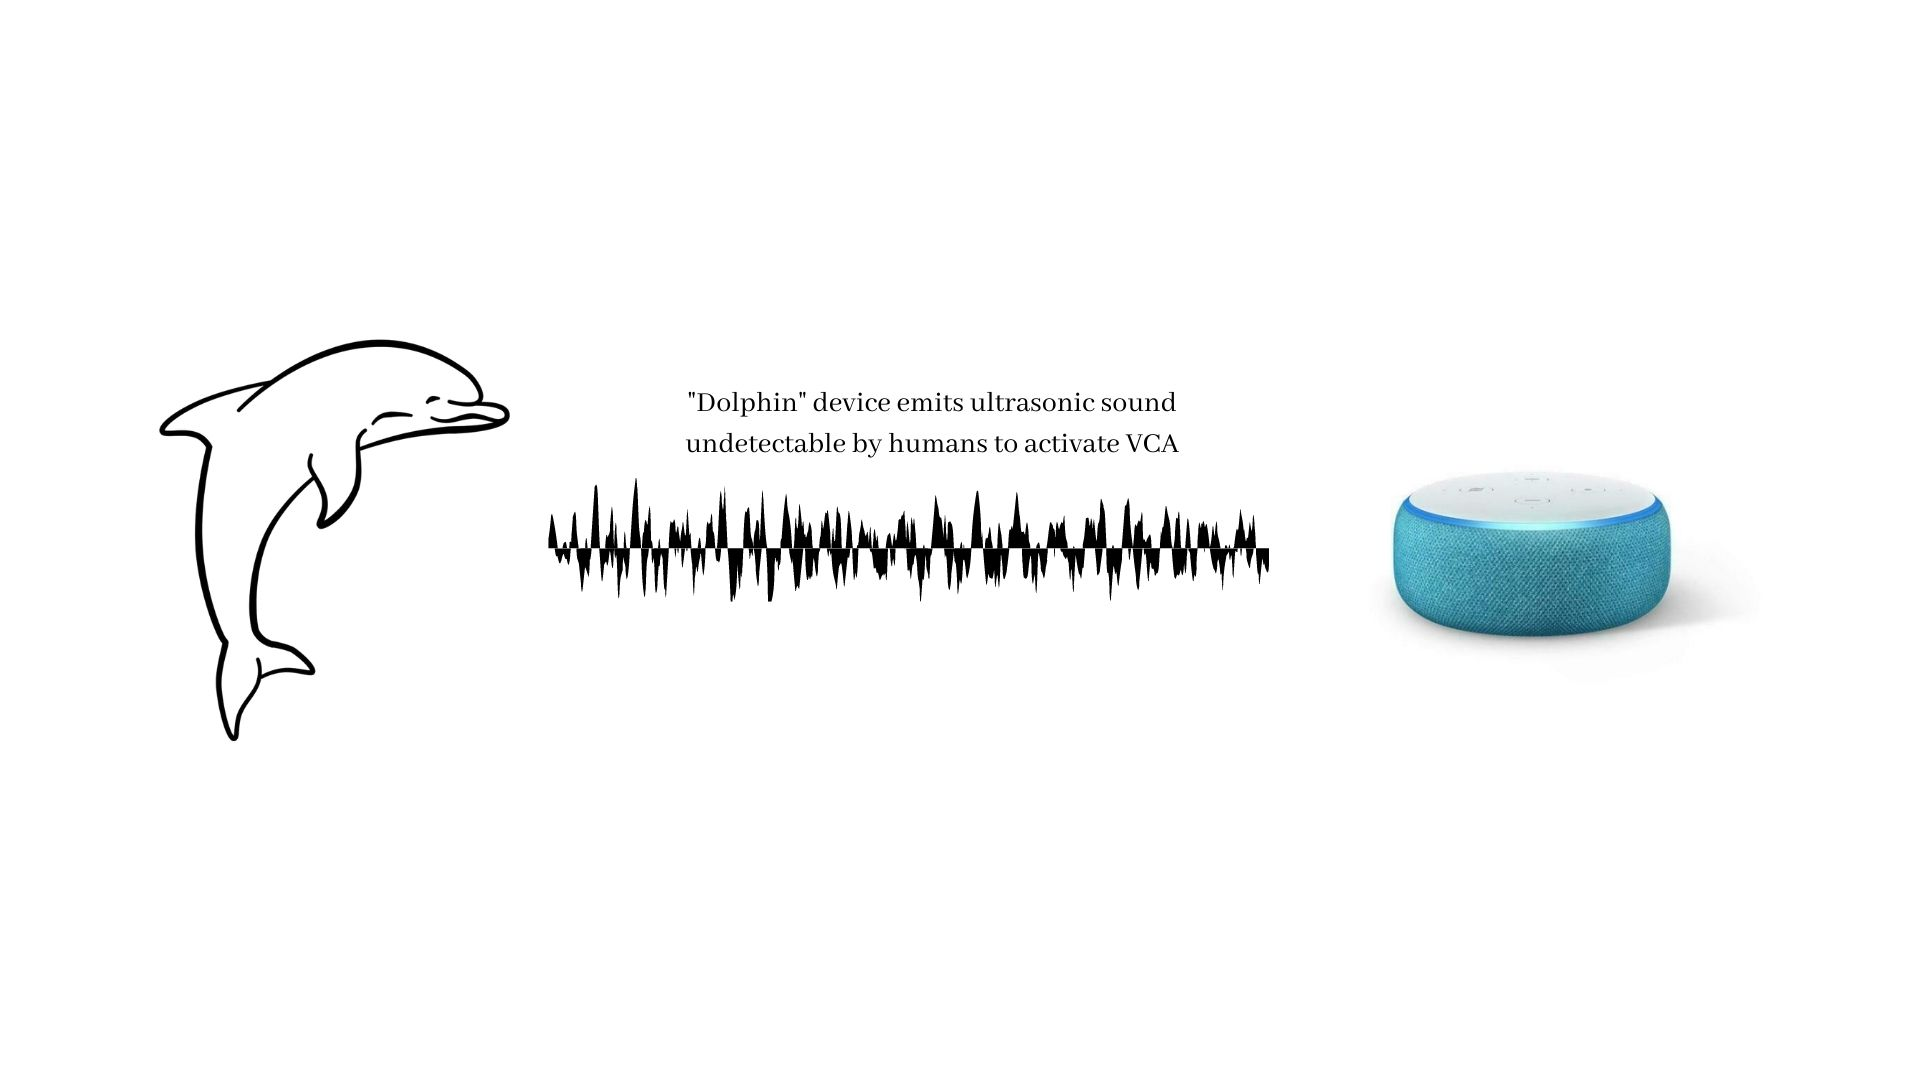
\includegraphics[width=\textwidth]{dolphinattack.jpg}
    \caption{Dolphin attacks utilize ultrasonic sound frequencies undetectable by the human ear.}
    \label{fig:dolphin}
\end{figure}

Other studies have found hardware issues in devices that could compromise user privacy and data. A study by Streiff et al. \cite{streiff:overpowered} shows that a smart toy by Fischer conceals an Android tablet motherboard. Researchers found that root access to the board was unprotected and that it was easy to gain access to both the camera and microphone built into the toy; it is entirely possible for an attacker to take advantage of this poor design to spy on other consumers.

Evidently, the industry has yet to fully understand each vulnerability that resulted through the widespread usage of IoT technologies. Our research aims to analyze two IoT products and develop a threat model for both, looking for vulnerabilities in their mobile applications, networks, and hardware.

\section{Children's Protection}
Under United States law, children's personal identifiable information is heavily protected under the Children's Online Privacy Protection Act (COPPA). When providing a service or product that is connected to the Internet to children under the age 13, developers are legally required to obtain parental permission and inform users of data collection. Data collection must be kept to a bare minimum for a product to function and collected data must be available for review and deletion.

Ever since COPPA was passed, many tools and resources were created to help developers implement extra measures for protecting children's data. For example, some software development kits (SDK) provide extra options to limit the kinds of data an application is able to collect \cite{reyes:coppa}, and Samet Privacy's kidSAFE\textsuperscript{\textregistered} Seal Program (fig. \ref{fig:kidsafe}) verifies the COPPA-compliance of devices and applications.

While meeting COPPA standards is a legal requirement for any Internet-connected product available in the United States, research has shown that developers often neglect doing so. Reyes et al. \cite{reyes:coppa} have found that out of the top 5,885 children's mobile applications on the Google Play Store analyzed in their study, a majority of them are potentially violating COPPA standards due to misuses of mobile SDKs. This discovery shows that although there are laws in place to ensures the safety of children's data, this industry has yet to fully accomodate for the requirements set through these laws. 

Another study conducted by Le et al. \cite{le:skillbot} delves into the safety of Amazon's VCA Alexa, which found that a few built-in applications, called \textit{skills}, that were designed for children harbored inappropriate contents and often collected too much data for COPPA-compliance. The study also found that many parents had concerns regarding the content of these \textit{skills} and often did not take full advantage of parental control features.

\begin{figure}
    \centering
    
\includegraphics[width=0.3\textwidth]{kidsafe1.png}
    
\includegraphics[width=0.3\textwidth]{kidsafe2.png}
    
\includegraphics[width=0.3\textwidth]{kidsafe3.png}
    \caption{The kidSAFE seal of certification helps parents identify Internet-connected products that are verifiably COPPA-compliant.}
    \label{fig:kidsafe}
\end{figure}

With the data and privacy of children at risk, it has become ever so important for developers to be wary of what data their products collect and what content is available to children. Finally, our study aims to find better methods of making data collection transparent and suggest implementing several mechanisms that can help ensure children's safety. 

% METHODOLOGY %%%%%%%%%%%%%%%%%%%%%%%%%%%%%%%%%%%%%%%%%%%%%%%%%%%%%%%%%%%%%%%%%%%%%%%%%
\chapter{Methodology}
\label{ch:methodology}
Our research delves into two separate fields. First, we explore end-user psychology through survey data. On the other hand, we also delve into the technical aspects of two existing IoT products that are currently available on the market: Amazon's Echo Dot for Kids is a voice assistant smart home device with parental control and restriction features, and the ROYBI Robot is a smart toy designed as a tutor for young children (fig. \ref{fig:devices}).

\begin{figure}
    \centering
    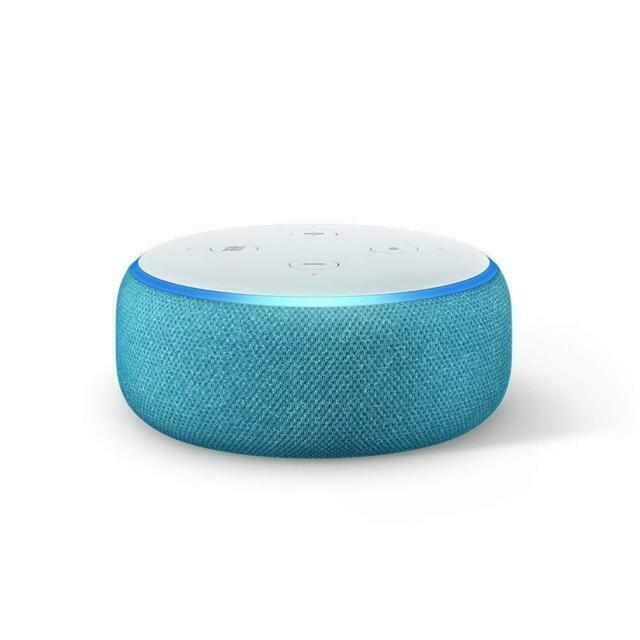
\includegraphics[width=0.3\textwidth]{echo.jpg}
    \includegraphics[width=0.3\textwidth]{ROYBI.jpg}
    \caption{Our research involves analysis of two smart devices designed for children: the Amazon Echo Dot for Kids and the ROYBI Robot.}
    \label{fig:devices}
\end{figure}

\section{End-User Study}
We want to understand the psychology involving, parents, IoT, and data privacy through developing a mental model.

\subsection{Privacy Policy}
Both devices presented in the survey have privacy policies to inform users of data collection and what rights the user has. Since devices designed for child-use must also comply with COPPA, we can expect to see specific details regarding specific permissions granted by the parents, what data is collected, and how much control parents have over collected data. We review each device's privacy policy and compare our findings from the device taxonomy to reveal any inconsistencies in data collection. We also look into any COPPA violations that could possibly be present in the devices.

\subsection{Survey}
To build a generalizable mental model on parents and IoT devices, we ran a survey (Appendix \ref{app:questions}) to better gauge the experiences and opinions of parents concerning smart devices designed for children. We ask questions regarding their experience with technology, thoughts on smart devices and smart toys, privacy practices, and demographics. Additionally, we show the subjects short videos demonstrating the two smart devices in our research and ask about their thoughts and concerns about them. 

Our survey was conducted through Qualtrics. The research was approved by the University of California, Santa Cruz (UCSC) Institutional Review Board (IRB) and abides by the regulation of the Office of Research Compliance Administration (ORCA). We collected no personal identifiable information except an email, which is deleted from our records as compensation is sent. Our subjects consisted of parents of children ages 6 or younger that are currently residing in the United States. We recruited participants from an existing subject pool from the Baby Lab at UCSC, as well as through word-of-mouth and email. Those who completed the survey were compensated with a \$10 Amazon gift card.

Through the questions asked on the survey, we aim to model several high-level properties of parents and IoT.

\subsubsection{Data Privacy}
As discussed in chapter \ref{ch:background}, previous research has shown that smart device users that are less experienced with technology tend to show less concern for data privacy. We ask questions regarding how our subjects keep their data safe and if they have any concerns regarding data collection in Internet-connected devices. These questions help us understand which data privacy issues parents are aware of and which issues may require additional scrutiny.

\subsubsection{Cloud Infrastructure}
We want to measure the level of understanding parents have for the cloud infrastructure of the two smart devices we present in the survey. We ask questions gauging the subjects' understanding of how data is collected through the devices, where it is stored, and how it is transferred over a cloud server. 

\subsubsection{Developer Reliability}
We also want to understand the extent to which parents trust the Internet-connected devices that are currently available on the market. We ask for the subject's opinions on the two devices presented in our research, such as what they liked or disliked about the toy and what kind of design improvements could be made. Understanding a parent's trust in children's IoT devices helps us further understand their security weaknesses and shines a light on what features parents are concerned about.

\section{Device Taxonomy}
In the technical aspects of our research, we look into two smart devices designed for children that are available on the market.

\subsection{Network Analysis}
In order to develop threat models for our devices, we investigate the security standards of these devices. Using the Internet Sharing feature on OSX, we used a Macbook as a WiFi endpoint for both devices, as well as a mobile device for the applications used to control them. The laptop connected to a router through an ethernet cable serves as a bridge between the router and our smart devices \ref{fig:experiment}. We then use Wireshark to analyze the network traffic of all of our devices. Details we are looking for include:

\begin{itemize}
    \item Frequency of packets being sent 
    \item Total bandwidth of network traffic 
    \item Servers the devices are in communications with 
    \item Packet protocol
    \item Encryption standards
    \item Possible attack vectors
\end{itemize}

All in all, we are searching for insecure features that may either violate COPPA standards or be an exploitable security flaw.

\begin{figure}
    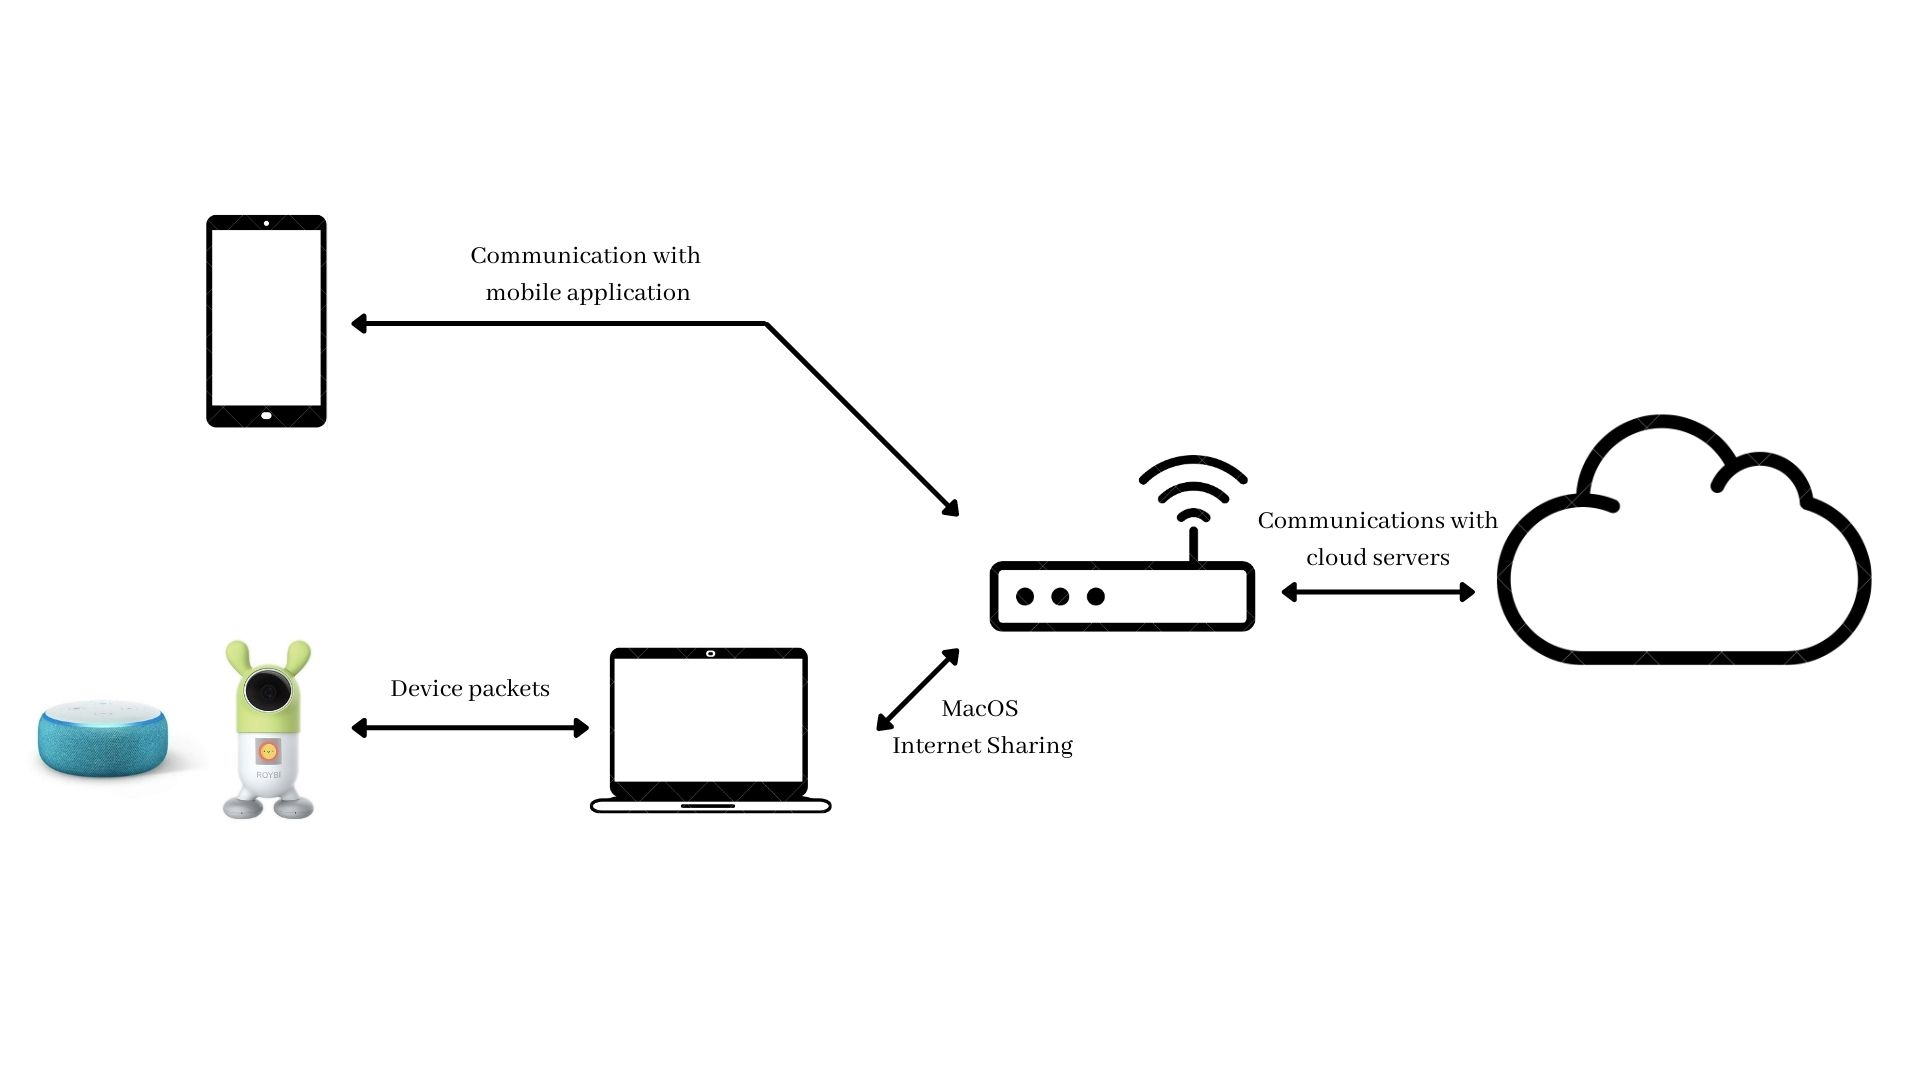
\includegraphics[width=\textwidth]{experiment.jpg}
    \caption{A high level overview of our experiment setup.}
    \label{fig:experiment}
\end{figure}

\subsection{Attack Vectors}
Given the versatility of both the Echo Dot and the ROYBI Robot, our research aims to find possible attack vectors for both devices. With the network analysis performed as described in the previous section, we first examine any inconsistencies with encryption protocols and packet patterns to find network exploits. We also examine each feature of both devices to observe any possible COPPA violations or privacy breaches. Finally, we test known attack vectors on the devices. 

The methodology presented in this chapter results in both a mental model of parents and their children's interactions with smart devices and a threat model of the possible attacks or breaches of privacy that could occur in smart device use. We seek to compare these two models in order to recommend changes to be made for a safer IoT environment.

% MENTAL MODEL %%%%%%%%%%%%%%%%%%%%%%%%%%%%%%%%%%%%%%%%%%%%%%%%%%%%%%%%%%%%%%%%%%%%%%%%
\chapter{End User Study}
\label{ch:mental}
We first investigate the end-user's experiences and perceptions of smart devices. In this section, we review the privacy policies for Amazon's Echo Dot for Kids and the ROYBI Robot, both of which are smart devices designed for children's use. Our goal is to first find if the products' privacy policies align with federal law and our expectations. We also analyze the survey data we collected on Qualtrics and compare it with the contents of the privacy policy to find whether the expectations of our subjects align with the policies the companies put in place.

\section{Privacy Policy}
\subsection{Amazon}
Amazon's privacy policy for Echo devices are spread across two separate documents. The first document presents information on privacy with Alexa and Echo devices. It states that the device only records audio after it detects the ``wake word'' that triggers voice commands. When a user speaks to Alexa, the Echo device's VCA, the device sends the audio recording to an Amazon cloud service where it is processed. Users have the ability to review and delete voice recording through the Alexa mobile application. This document also clarifies that voice recordings are used to improve Alexa's natural language processing capabilities, where a human reviews a small sample of all recordings to assist in supervised machine learning \cite{supervised}. Users can manage the usage of their voice recordings.

The second document pertains to children's privacy. It states that if a parent or guardian consents, Amazon may collect personal information such as name, birthdate, contact information, voice, photos, videos, location, and device identifiers such as IP addresses or cookies. Amazon uses this collected information to ``improve products and services, including personalizing offerings and recommendations for children, communicating information, enforcing parental controls, and giving parents visibility into how their children use [their] products and services''. Children will not receive interest-based advertisements based on collected data, and data is only shared in transactions and services of third parties, business transfers, and for the protection of Amazon. The parent or guardian may choose to revoke data collection permissions at the cost of some services and features.

\subsection{ROYBI}
ROYBI's privacy policy contains information on data collection, third parties, and user rights. The document states that upon creating an account, the service collects the user data of both guardian and child, including name, birthday, gender, email address, password, and usage data. Furthermore, with parent or guardian approval, the service also collects audio and video recordings during the child's lesson. Any information collected will not be shared for marketing purposes, but may be shared with service providers (Amazon AWS, Google Play Store or App Store transactions), disclosed under court order, transferred through a company merger or acquisition, or displayed as a testimonial as a satisfied adult user. 

Because the ROYBI Robot is specifically designed for children's use, the privacy policy contains a section dedicated to COPPA compliance. The document specifies that ROYBI does not knowingly allow children under the age of 13 to use their services without a parent or guardian's consent. The privacy policy also promises that all collected information is securely stored within a database and currently is not used for third-party advertising purposes. All video, audio, and password data are sufficiently encrypted and user data is only accessible by the users themselves. In the event of a data breach, ROYBI will inform users by email. Users are also able to close their accounts, in which their data will be kept in the database for at most 90 days.

\section{Survey Data}
In our survey, we asked questions pertaining to general demographics, developer reliability, data privacy, and understanding of cloud infrastructure. 

\subsection{Demographics}
We collected anonymous data from 16 parents with children ages 6 or younger. Our participants ranged from 26 to 64 years old and had between 1 and 3 children. They held a wide variety of occupations, although only four reported a technical-based job. We asked our participants about their experience with technology. While self-reported experience does not necessarily reflect actual experience, we combine this and the occupation as a rough indicator of their knowledge. Table \ref{table:demographics} shows the data that we have collected and assigns an identifier to each participant.

\begin{table}
    \centering
    \begin{scriptsizetabular}{|c|c|l|l|l|}
        \hline 
        ID & Age & Children's Age(s) & Occupation & Familiarity with Technology (Self-reported) \\
        \hline
        A & 43 & 4 & Data Analyst & Professional Experience\\
        B & 42 & 6 & Accountant & Some Experience\\
        C & 45 & 6 & Data Analyst & Some Experience\\
        D & 37 & 2 & Sales & Moderate Experience\\
        E & 37 & 1, 3 & Homemaker & Lots of Experience\\
        F & 42 & 3, 4 & Quality Specialist & Some Experience\\
        G & 39 & 5 & Coordinator & Lots of Experience\\
        H & 48 & 5 & Clinical Pharmacist & Professional Experience\\
        I & 39 & 4, 6 & Construction Superintendent & Professional Experience\\
        J & 39 & 0, 3 & Physical Therapist & Some Experience\\
        K & 38 & 4, 6 & Teacher & Professional Experience\\
        L & 38 & 2, 4 & None & Moderate Experience\\
        M & 39 & 3 & Lawyer & Lots of Experience\\
        N & 64 & 4 & Mathematician & Professional Experience\\
        O & 35 & 1 & Software Engineer & Professional Experience\\
        P & 26 & 0, 2, 4 & Direct Sales & Lots of Experience \\
        \hline
    \end{scriptsizetabular}
    \caption{Demographics data collected from our Qualtrics survey.}
    \label{table:demographics}
\end{table}

\subsection{Developer Reliability}
\subsubsection{Smart Device Experience}
In the survey, we asked the participants about their own experiences with IoT devices. We first ask about smart home devices and other smart devices separately; we found that 10 out of 16 participants have owned a smart home device for more than two years and 13 participants have owned smart devices for more than 2 years. Table \ref{table:smartdevices} draws the collected data.

Of the participants that owned smart home devices, 10 allow their children to use it. For other smart devices, 7 of 13 smart device owners allow their children to use it. We have found that there have been many reasons to allow or disallow it. For example, participant M states that they allow their oldest child to use their smart television device since it ``works like any TV''. Participant O, who works in software engineering, showed distrust for these devices, data collection, and potential attacks.

\begin{table}
    \centering
    \begin{scriptsizetabular}{|c|l|l|l|l|l|}
        \hline 
        ID & Smart Home Owner & Child Smart Home Use & Smart Device Owner & Child Smart Device Use \\
        \hline
        A & More than 2 years & No  & More than 2 years  & Yes\\
        B & More than 2 years & Yes & 1-2 years          & No\\
        C & More than 2 years & No  & N/A                & N/A\\
        D & N/A               & N/A  & More than 2 years & No\\
        E & More than 2 years & Yes & More than 2 years  & No\\
        F & N/A               & N/A & More than 2 years  & No\\
        G & More than 2 years & Yes & More than 2 years  & Yes\\
        H & More than 2 years & Yes & More than 2 years  & Yes\\
        I & More than 2 years & Yes & More than 2 years  & Yes\\
        J & More than 2 years & Yes & More than 2 years  & No\\
        K & 1-2 years         & Yes & Less than 3 months & Yes\\
        L & 1-2 years         & Yes & More than 2 years  & No\\
        M & More than 2 years & No  & More than 2 years  & Yes\\
        N & 1-2 years         & Yes & More than 2 years  & No\\
        O & N/A               & N/A & More than 2 years  & Yes\\
        P & More than 2 years & Yes & More than 2 years  & No\\
        \hline
    \end{scriptsizetabular}
    \caption{Data collected from participants of smart device ownership and child use.}
    \label{table:smartdevices}
\end{table}

\subsubsection{ROYBI Robot}
The participants are shown a demonstration video about the capabilities of the ROYBI Robot and are asked to answer a few questions about their thoughts on the device. We found that not a single participant has heard of this device. While some of them liked the toy's interactive capabilities, most of the feedback we received was negative. For one, several participants responded with complaints about the product design; the screen was too small and ROYBI's voice sounds too unnatural. Many participants also expressed concern for their child's safety. Participant D had concerns with how the camera is used and the possible threat of hackers, and participant O disliked the use of facial recognition altogether.

When asked whether the participants would consider purchasing the ROYBI Robot, those who answered ``yes'' were interested in its capabilities in teaching languages or were looking for interactive at-home learning, as our research was conducted during the COVID-19 pandemic. On the other hand, those who answered ``no'' either already own an alternative device or disliked the product design.
When asked about the contents of the device's privacy policy, 7 participants were not sure or did not care. Of those who responded otherwise, participants mentioned restrictions against video, image, audio, and other forms of data collection. Many answers expected that no data is collected whatsoever while some answers specifically talked about preventing the collection of identifiable personal information. Participant O expected ``explanations of what computation happens on the device or on the cloud [and] explanations of what data is stored''.

\subsubsection{Echo Dot for Kids}
Similarly to the previous section, we showed another demonstration video for our second subject device, Amazon's Echo Dot for Kids, and asked for the participants' opinions. 11 of our 16 participants have heard about the device, and several already own one. Positive opinions include comments about the design, ease of use, and parental controls. As for negative opinions, a common answer we found pertained to privacy issues as participants expressed concerns for the device's ability to evesdrop and collect information while idle. Other responses showed adversity to voice controlled assistant technology as a whole. 

Since many of our participants already owned an Echo device, there is no need for them to purchase another. Some considered buying one because of the provided convenience and entertainment, while those who were not considering purchasing the device did not think it was a necessary addition to their homes. When asked about the device's privacy policy, the responses were very similar compared to ROYBI's expectations. While some participants did not know or care, others expected that no recordings are saved or that personal information is not shared with third parties. Many of the responses held resentment towards privacy in technology; participant D states that they ``don't believe tech cares about privacy'' and participant N expects ``usual meaningless nonsense''.

%use Q36
\subsection{Data Privacy}
\begin{table}
    \centering
    \begin{scriptsizetabular}{|l|l|l|l|l|}
        \hline 
        Question & Disagree & Slightly Disagree & Slightly Agree & Agree \\
        \hline
        \begin{scriptsizetabular}{@{}l@{}}
            I have concerns for how my data \\
            is collected and stored on the Internet.
        \end{scriptsizetabular} & 0 & 4 & 4 & 8 \\ &  &  &  & \\
        \begin{scriptsizetabular}{@{}l@{}}
            I find it important that collected data is kept private.
        \end{scriptsizetabular} & 0 & 2 & 4 & 10 \\ &  &  &  & \\
        \begin{scriptsizetabular}{@{}l@{}}
            I thoroughly research into Internet-connected \\
            devices before making a purchase.
        \end{scriptsizetabular} & 1 & 3 & 7 & 5 \\ &  &  &  & \\
        \begin{scriptsizetabular}{@{}l@{}}
            I am familiar with the Children's\\ 
            Online Privacy Protection Act (COPPA).
        \end{scriptsizetabular} & 8 & 2 & 4 & 2 \\
        \hline
    \end{scriptsizetabular}
    \caption{Responses to the scale questions in our survey pertaining Internet safety.}
    \label{table:scale}
\end{table}

We presented statements regarding data privacy and COPPA and asked participants on whether they agree or disagree with the statement on a scale (table \ref{table:scale}). We found that no participants fully disagree with the statements, ``I have concerns for how my data is collected and stored on the Internet'' and ``I find it important that collected data is kept private''. This shows that all participants, at the very least, are aware that data collection is an issue in technology. A majority of them answered ``Agree'', expressing real concern for these issues at hand. 12 participants agreed and slightly agreed with the statement, ``I thoroughly research into Internet-connected devices before making a purchase'', demonstrating some skepticism in IoT technologies. Inversely, a majority of participants did not express familiarity with COPPA; in general, without a technical background, it may be more difficult to understand how personal data is stored and why collecting children's data requires more caution. 

When presented with a list of security concerns regarding devices connected to the Internet, we found that participants were most concerned about general privacy and data storage (table \ref{table:privacyconcerns}). Since many modern devices must be kept on, a common concern is that users do not know what data is being recorded, when they are recording, and how the data is being transported and stored. When asked to elaborate on the selections made, participant F states, 
\begin{quote}
    ``We worry after hearing those stories of these devices recording at all times. We have thought of buying the Alexa or Google Home devices for the convenience and fun, but always stop ourselves due to fear of privacy loss.''
\end{quote}


%Q37
\begin{table}
    \centering
    \begin{scriptsizetabular}{|l|c|}
        \hline 
        Security Concern & Count \\
        \hline
        Data Storage & 10\\
        Data Usage & 6\\
        Inappropriate Content & 8\\
        Privacy & 12\\
        Other & 1\\
        None & 1\\
        \hline
    \end{scriptsizetabular}
    \caption{Responses pertaining security concerns that participants have regarding Internet-connected devices from a multiple choice form.}
    \label{table:privacyconcerns}
\end{table}

When presented a list of concerns regarding the dialogue between children and smart devices, most participants were primarily concerned about the privacy of the conversations and how collected data is used (table \ref{table:dialogue}). In particular, many participants elaborated that they are concerned with how collected data could affect their children in the future. Participant O says,
\begin{quote}
``What data about my child is being collected, for seemingly innocuous reasons, maybe by people who don't have kids and don't have concerns about data... how is all this data about my child possibly going to come back and haunt them later in ways we can't even comprehend now?''
\end{quote}
From our data, we found that most concerns from our participants stem from not knowing when and what data is collected. Other concerns included worries of data theft, data sharing with third parties, preventing advertisement influence, and whether device content is child-friendly.

%Q39
\begin{table}
    \centering
    \begin{scriptsizetabular}{|c|c|l|l|l|}
        \hline 
        Dialogue Concerns & Count \\
        \hline
        Inappropriate Dialogue & 4\\
        Data Storage & 4\\
        How data is used & 11\\
        Privacy of Conversations & 11\\
        Other & 0\\
        None & 4\\
        \hline
    \end{scriptsizetabular}
    \caption{Responses pertaining to concerns of the dialogue between children and smart devices.}
    \label{table:dialogue}
\end{table}

Finally, we ask the participants about the practices that their families use to keep their data safe. Some solutions include avoiding suspicious URLs, using a firewall, using multi-factor authentication \cite{mfa}, using unique passwords, and avoiding smart devices altogether. Some participants admitted to not following any form of security practices on the Internet.

\subsection{Cloud Infrastructure}
We ask questions pertaining to the participant's understanding of how an IoT device works in a cloud infrastructure. First, we asked participants to describe their understanding of how data collection works in Internet-connected devices. While only 3 responses mentioned cloud services, a majority of participants believe that IoT devices do collect and save data in some capacity. Many responses also mentioned that search engines, social media services, and mobile applications collect data through search queries and usage statistics as well. 3 participants were unable to answer the question and responded with, ``I don't know''.

Second, we ask participants to describe their understanding of how data is stored after being collected. We found that half of the participants talked about the cloud or servers over the Internet; participant O specifically mentioned Amazon's S3 cloud storage service. The rest of the participants did not know where collected data is kept or guessed that it was saved within the device itself.

Finally, we ask our participants to describe any concerns they have for how their data is stored on the Internet. Almost every participant shared grievances about the increase in data collection in recent years. Several responses expressed concerns in possible data breaches that could expose their personal identifiable information. Many responses disliked the fact that data can be hard to delete and could be used against them in the future. Participant K found that targeted advertisements helped them find suitible products but still expressed concern over voice recording collection. Many participants are also worried about companies selling their data for profit.

\section{Mental Model}
From the data we collected from survey participants and privacy policy review, we can form a generalizable mental model for smart device users. We found that while most users know about or have heard of the importance of data privacy, they do not necessarily have the background knowledge to understand the full scope of the issue. Those who have a background in a technical field have demonstrated a deeper understanding of how data is collected, where it is stored, and the consequences of a privacy breach. However, those who do not often undermine the severity of these consequences and follow fewer security practices to keep their data safe.

We have also found that user expectations on what would be on a device's privacy policy often does not match with the actual contents. While many of our participants showed concern in companies selling their data for profit, we have found that neither of the devices we analyze in our research directly sell any data to third-parties. A majority of our participants have also expressed concerns with data collected through microphones on smart devices. However, Amazon's Echo device privacy policy clearly states that it only records audio after it detects the user's chosen trigger word. ROYBI's policy states that audio and video data are only recorded during lessons.

Furthermore, we found that the design of a product affects a potential buyer's perceptions. Participants found that the ROYBI Robot's design was crude and thus showed more uncertainty towards its security. With the addition of a camera, a microphone, and facial recognition capabilities, many of the participants expressed concerns towards the data the device collects from children. On the other hand, the Echo device's ease of use, as well as Amazon's reputation, earned the trust of our participants, who showed more desire to purchase one.

% TAXONOMY %%%%%%%%%%%%%%%%%%%%%%%%%%%%%%%%%%%%%%%%%%%%%%%%%%%%%%%%%%%%%%%%%%%%%%%%%%%%
\chapter{Device Taxonomy}
\label{ch:taxonomy}
We perform network analyses on two separate products: Amazon's Echo Dot for Kids and the ROYBI Robot, both of which are smart devices designed for children's use. In our analyses, we pay attention to each feature the devices offer and how they communicate with their cloud services and the parent's mobile device through its designated mobile application.

\section{Amazon Echo Dot for Kids}
The Amazon Echo Dot is a smart home device with Amazon's VCA, Alexa, built in. Although marketed differently, there are currently no hardware differences between the Echo Dot and the Echo Dot for Kids. Instead, Amazon FreeTime, which can be enabled for any Amazon Echo device, adds additional parental control features. Enabling FreeTime automatically filters any explicit phrases and \textit{skills} from the device; parents are able to set daily usage limits and moderate what Alexa \textit{skills} are available to their children. Parents can also create profiles for multiple users to assign devices to different children.

\subsection{Network Analysis}
\subsubsection{Echo Dot Device}
We use the experiment setup as described in figure \ref{fig:experiment} to capture packets from the Echo Dot and the mobile device. We have found that on startup, the device initiates several DNS queries for various subdomains of the following:
\begin{itemize} 
    \item \texttt{amazon.com}
    \item \texttt{amazonaws.com}
    \item \texttt{fireoscaptiveportal.com}
    \item \texttt{amazonalexa.com}
    \item \texttt{amcs-tachyon.com}
    \item \texttt{cloudfront.net}
\end{itemize}
All of these domains are either owned or registered by Amazon. 

Upon receiving a DNS response, the device establishes a connection with the aformentioned servers using the TLS 1.2 protocol and communicates with them through TCP. All packets are encrypted and all subsequent communications use the same protocols.

When inactive, the device intermittently communicates with a database endpoint at \\\texttt{spectrum.s3.amazonaws.com}, sending a small number of TCP packets every 20 seconds. The Echo Dot's begins to listen when a trigger word is detected; by default, this is set to ``Alexa''. The device itself simply records a voice command and sends it to Amazon's Alexa Voice Services API to be parsed \cite{alexa}. The API then responds with an appropriate action. If any settings are changed, they are reflected in Amazon's cloud servers and the mobile application (fig. \ref{fig:voicecom}). Users are also notified by email when Alexa settings have been changed.

\begin{figure}
    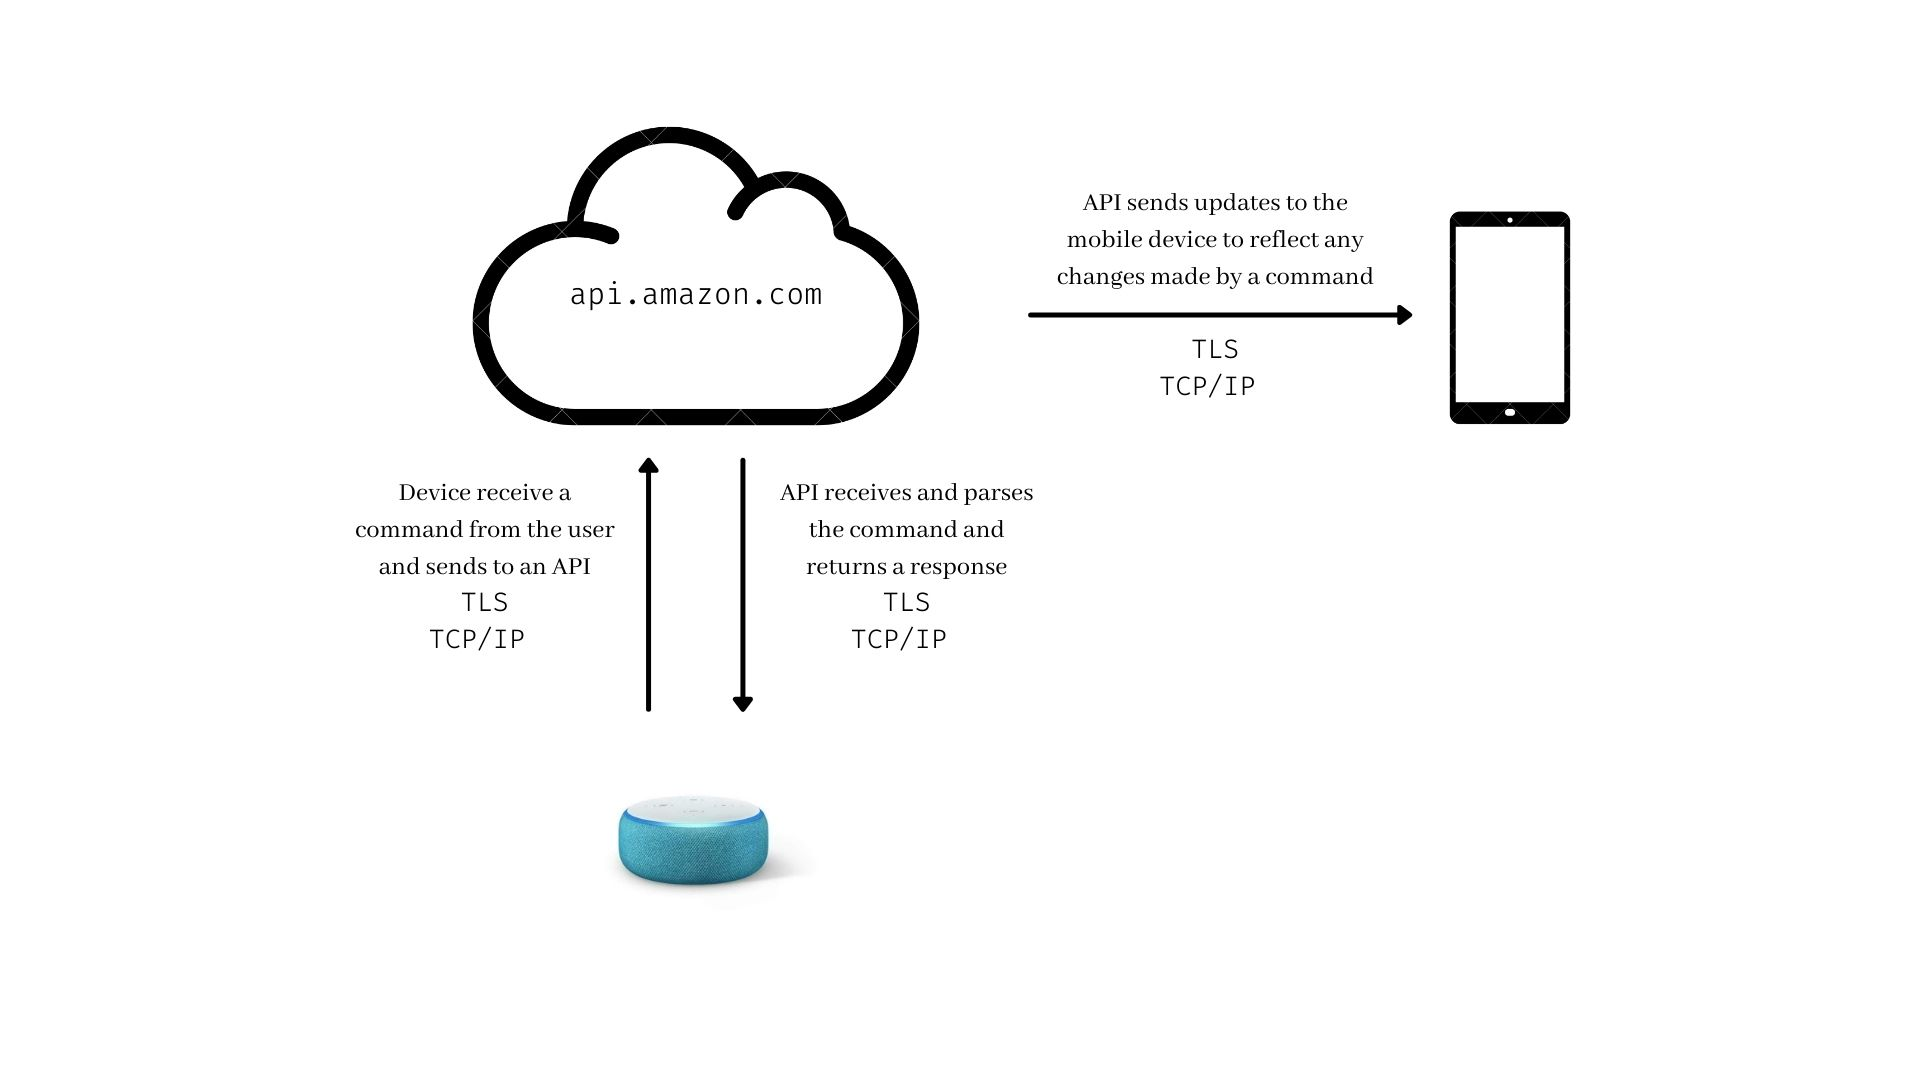
\includegraphics[width=\textwidth]{voice command.jpg}
    \caption{Upon invoking a voice command, the Echo Dot records it and sends it to a cloud server. The server parses the command and responds with an appropriate action, and any changes made will be reflected in the server and the mobile application.}
    \label{fig:voicecom}
\end{figure}

Feature usage network bandwidth differs depending on what command is invoked. A simple ``Alexa, what time is it?'' sends and receives 131 KB of packets over 202 packets in 6 seconds, while commands that invoke Alexa \textit{skills} may use upwards of several MBs, depending on its complexity. Furthermore, third-party skills require third-party servers. For example, invoking the ``Disney Stories'' skill requires a communication establishment with \texttt{alexastoryassets.content.disney.io}, which is not managed by Amazon.

\subsubsection{Alexa Mobile Application}
The Alexa mobile application is available on both the Apple App Store and the Google Play Store. From here, Echo device users can use it to set up the device, connect it to a WiFi network, and access a myriad of features and settings, including FreeTime. Network analysis reveals that the application communicates with the same set of servers as the Echo device, except \texttt{fireoscaptiveportal.com}. All packets are well encrypted and use either the TLS 1.2 or TCP protocol, with the exception of Voice over Internet Protocol (VoIP) features that involves STUN and UDP streams to a server.

% Probably look into these figures again. UDP, STUN, cloud server name probably just say "amazon cloud"
\begin{figure}
    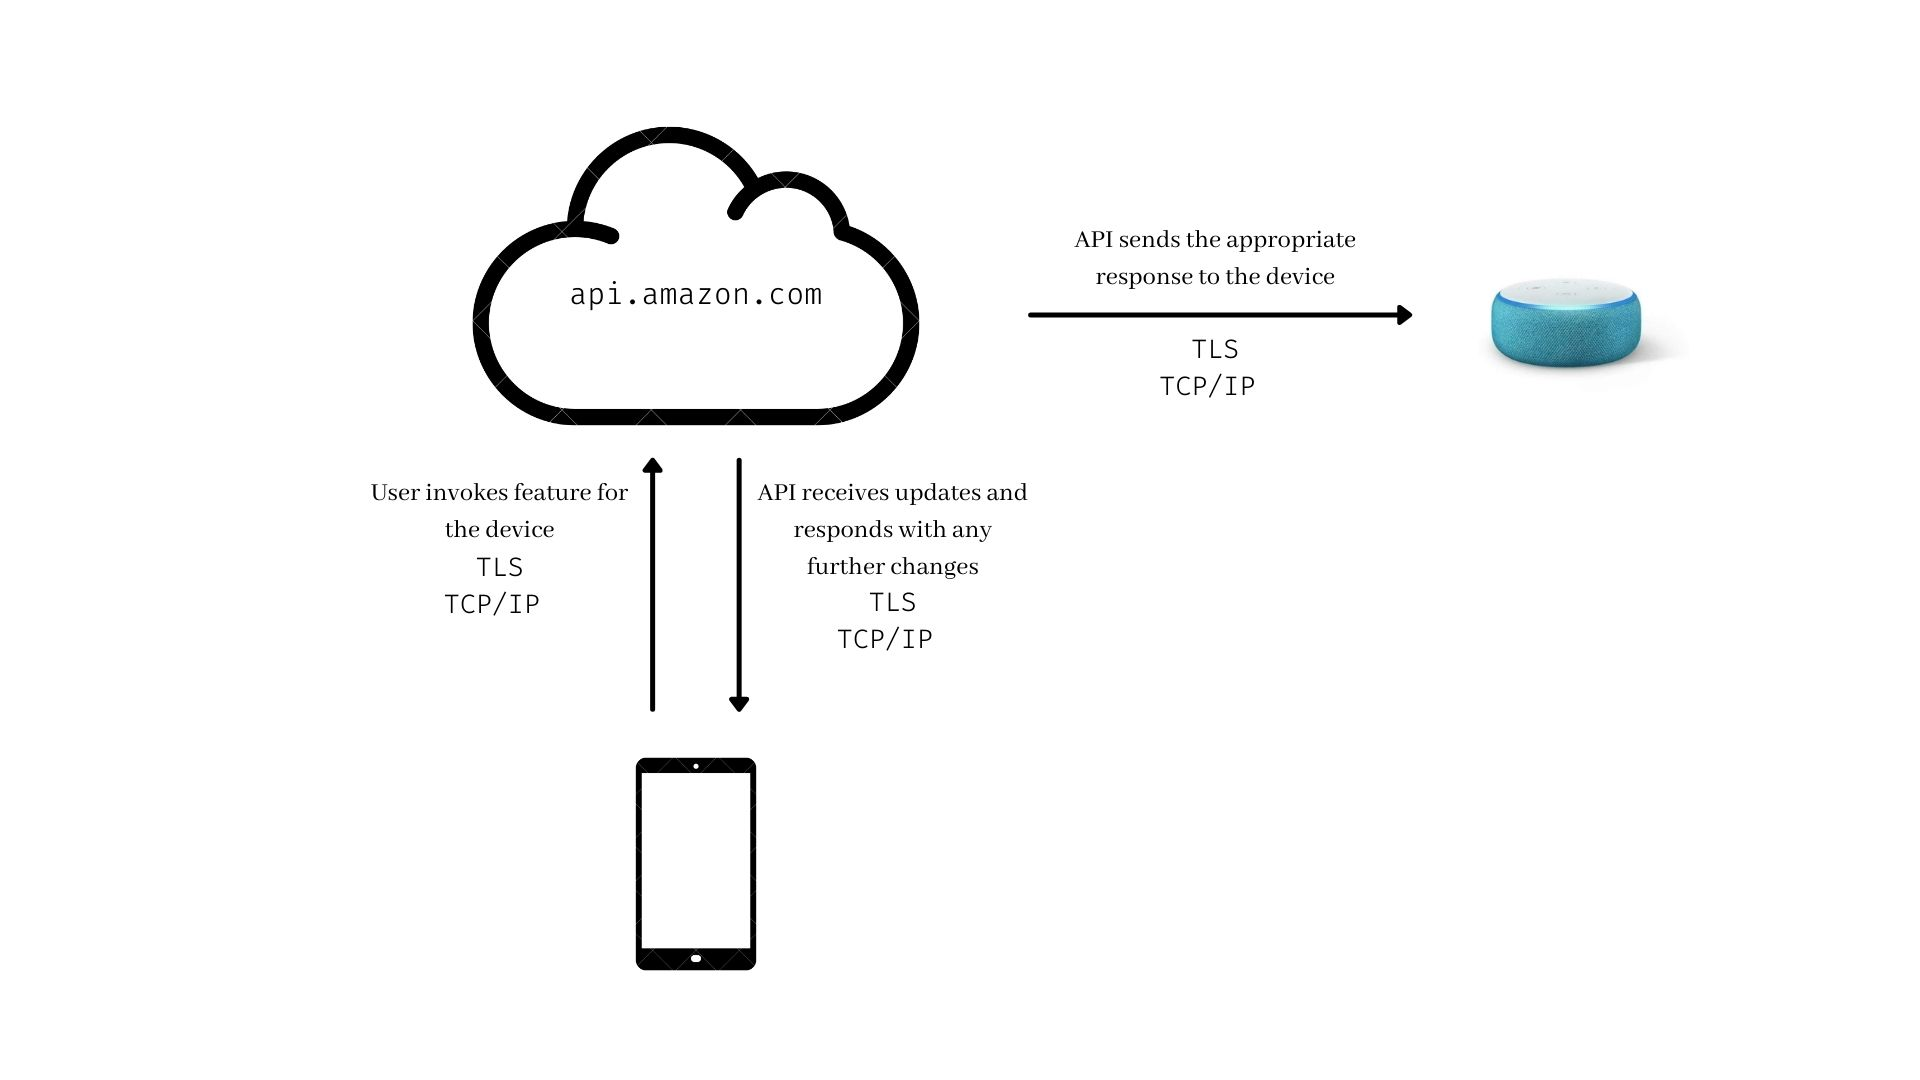
\includegraphics[width=\textwidth]{mobile command.jpg}
    \caption{If a mobile command is to be redirected to an Echo device, the API sends an appropriate action to the device. Any changes made within the server is updated on the application.}
    \label{fig:mobilecomm}
\end{figure}

We have found that FreeTime settings sufficiently filters explicit content and \textit{skills} from devices. When asking explicit questions involving violence, sexual content, Alexa will answer differently compared to when FreeTime is disabled, censoring explicit words and refusing to answer explicit questions. All \textit{skills} that contain explicit content are also disabled on devices with FreeTime enabled.

We review four features that directly interact with an Echo device:
\begin{enumerate}
\item Call: Requests a VoIP connection with an Echo device from mobile application
\item Drop In: Forces a VoIP connection with an Echo device from mobile application
\item Announce: Announces a typed message through an Echo device
\item Play: Plays music through an Echo device
\end{enumerate}

When a user invokes a feature on the application for the Echo device, one of two behaviors occur. If the feature does not involve VoIP, the application sends packets to a server, which then processes the command and redirects a response to the device (fig. \ref{fig:mobilecomm}). Depending on the feature, the application contacts different servers and APIs; table \ref{table:alexa} contains each feature relevant to the Echo Dot and what service is called. For features that do use VoIP, the devices establish STUN binding requests to a server. From here, the mobile device sends and receives STUN streams from said server, while the Echo device uses UDP streams. All STUN and UDP packets are well encrypted.

\begin{table}
    \centering
    \begin{scriptsizetabular}{|c|c|c|}
        \hline 
        Feature & Mobile Endpoint & Device Endpoint \\
        \hline
        Call & \begin{scriptsizetabular}{@{}c@{}}device-metrics-us-2.amazon.com \\ cmds-tachyon.com (STUN)\end{scriptsizetabular} & \begin{scriptsizetabular}{@{}c@{}}avs-alexa-14-na-amazon.com \\ cmds-tachyon.com (UDP)\end{scriptsizetabular} \\
        \hline
        Drop In & cmds-tachyon.com (STUN) & cmds-tachyon.com (UDP) \\ 
        \hline
        Announce & tp.cb7933e1d-frontier.amazon.com & avs-alexa-14-na-amazon.com \\ 
        \hline
        Play & tp.5fd53c725-frontier.amazon.com & Depends on \textit{skill} invoked \\
        \hline
    \end{scriptsizetabular}
    \caption{A list of features available on the Alexa mobile application that directly interacts with the Echo device.}
    \label{table:alexa}
\end{table}

\subsection{Echo Dot Attack Vectors}
While our network analysis for the Echo Dot shows that Amazon consistently utilizes state-of-the-art encryption and security standards, there are still some inherent risks involving smart home use. In this section, we discuss some of the possible attacks or data breaches that are possible due to the device's protocols. 

\subsubsection{Phishing}
If a user's account details are somehow compromised through phishing \cite{phishing}, it is possible for an attacker to access and modify all existing Alexa settings for the user's devices. Using a separate mobile device, we were able to download the Alexa application and log into our existing Amazon account. From here, we are able to access all information, features, and settings for the Echo Dot devices. In an adversarial situation, an attacker can change the settings in FreeTime or disable it entirely, talk through an Echo device using the Call feature, access child information, and overall can alter anything in the Amazon account.  

However, the Alexa application has a few security mechanisms implemented to prevent credential stuffing attacks. Attackers are only able to attempt to log in twice before they are required to complete a CAPTCHA \cite{captcha} challenge to continue. Additionally, upon any changes to the settings in an Alexa account, the owner is notified by email, giving them an opportunity to secure their accounts when they find suspicious activity.

\subsubsection{Home Occupancy}
If an attacker has access to the same network the device is connected to, they are possibly able to detect when an Echo Dot device has been activated. Because of the 20-second intermittent packets, any other outgoing packets can be an indication of a person present in the house. This information is often used by burglars when picking a house to rob; approximately 72\% of house robberies occur when no members of the household are present such as to avoid confrontation during the job \cite{burglar}. 

\section{ROYBI Robot}
The ROYBI Robot is an Internet-connected smart toy designed as a tutor in technology, math, science, and language arts for children. Parents and caretakers can schedule or play lessons through the mobile application on the ROYBI device to teach their children about various topics. The device and cloud system also have ``smart'' features, such as facial recognition and natural language processing.

\subsection{ROYBI Robot Network Analysis}

\subsubsection{ROYBI Robot Device}
Again, we use the experiment setup in figure \ref{fig:experiment} to capture packets from both the ROYBI device and the mobile application. Similarly, upon startup, the ROYBI device makes several DNS queries to the following domains and subdomains:

\begin{itemize}
\item \texttt{roybirobot.com}
\item \texttt{amazonaws.com}
\item \texttt{tencentcloudapi.com}
\item \texttt{time.pool.aliyun.com}
\end{itemize}

A majority of packets are sent to and from services hosted on Amazon Web Services, primarily at \texttt{iot.roybirobot.com} and \texttt{cdn.roybirobot.com}. Although the device also contacts Chinese web services, we found that only a small number of ICMP protocol packets were sent, likely for diagnostic reasons. When idle, the device sends a stream of TCP and TLS 1.2 packets to subdomains of either \texttt{roybirobot.com} or \texttt{amazonaws.com} every five seconds. Each of these packets are well encrypted.

The ROYBI device has a built-in camera and microphone with multiple functionalities. With parental consent, ROYBI can recognize a child's face, given a picture for reference through the mobile application. When the child is visible to the device, ROYBI retrieves a quip to communicate with the child. Parents can also access the camera and microphone directly through the application, which we analyze in the next section. The packaging comes with a rubber camera cover in case users have privacy concerns. 

\begin{figure}
    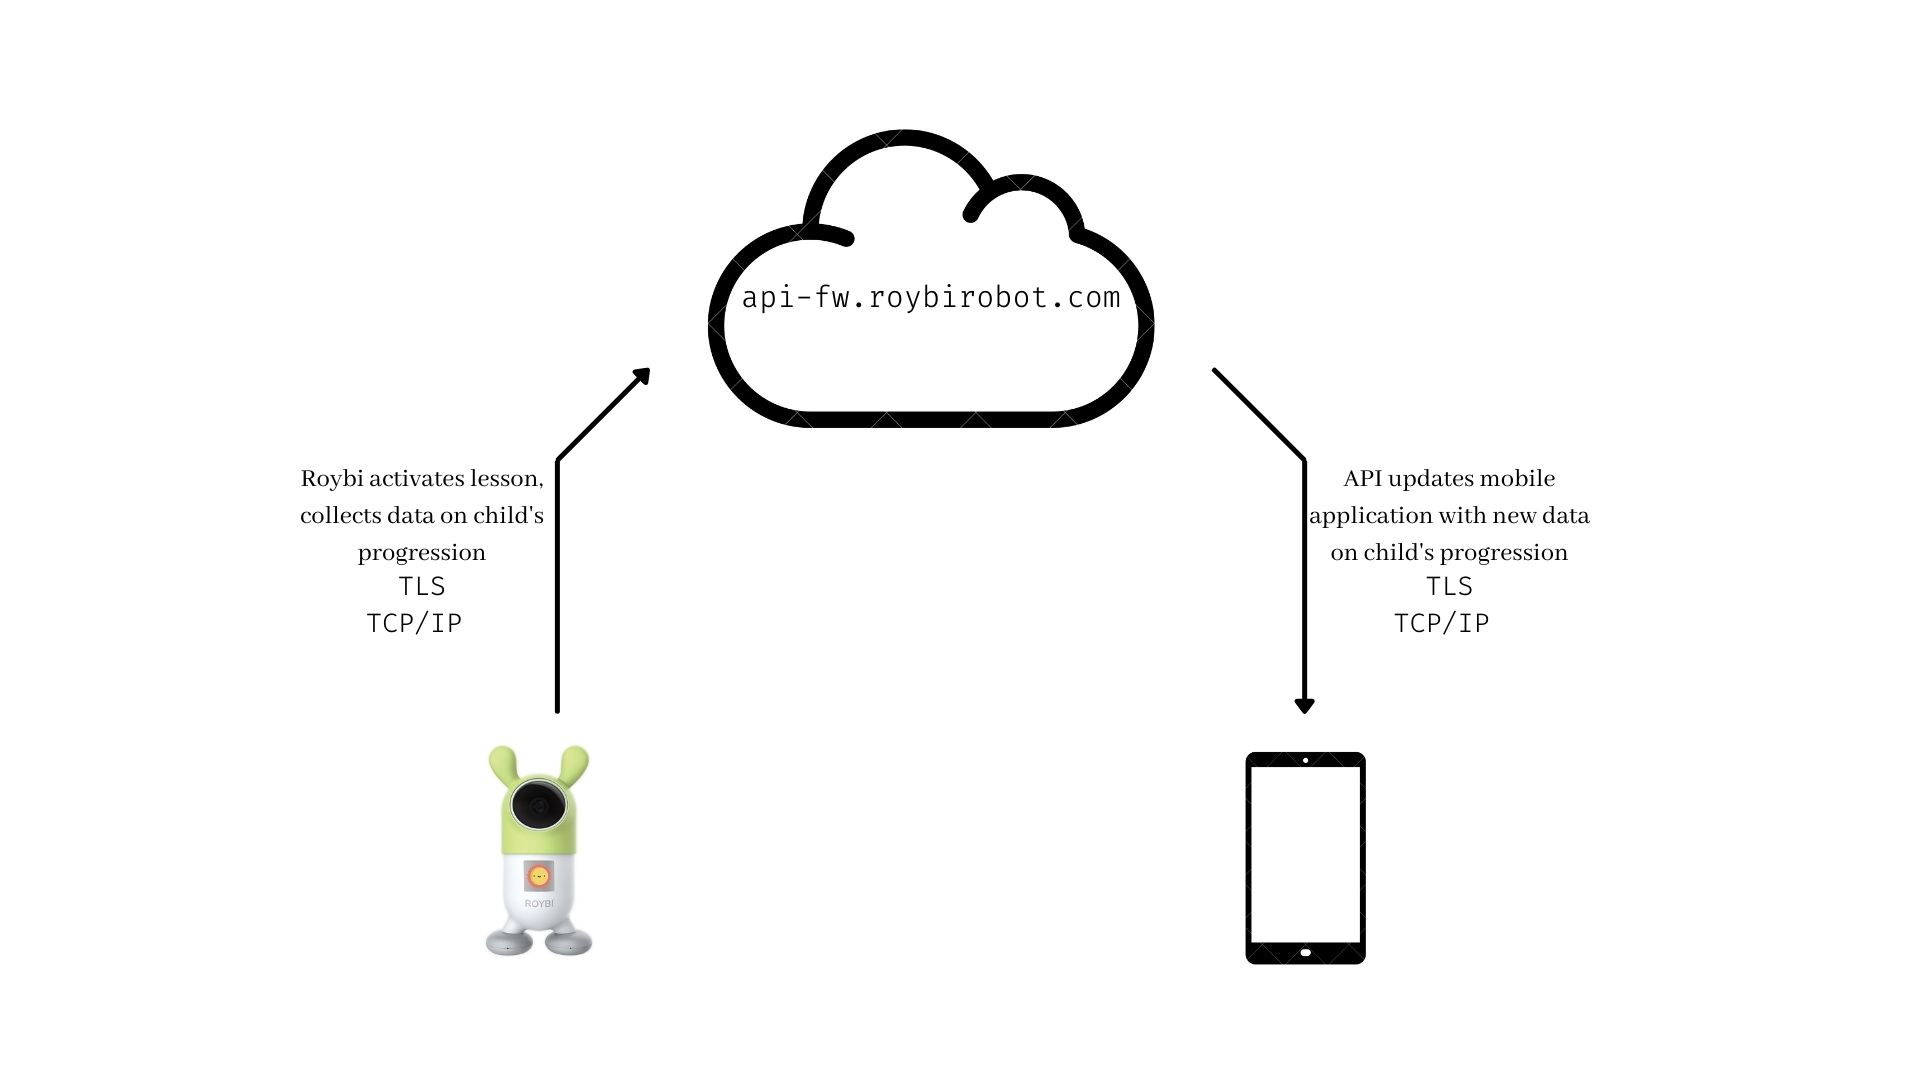
\includegraphics[width=\textwidth]{lesson.jpg}
    \caption{When ROYBI starts a lesson, the device downloads lesson data, tracks the student's progression, and updates the child's progress report.}
    \label{fig:lesson}
\end{figure}

Primarily, the camera and microphone are used during lessons. When a new or scheduled lesson is started, the device exchanges packets with \texttt{roybirobot.com}, presumably to download lesson data. During the lesson, for each response, the device exchanges packets with the cloud servers (fig \ref{fig:lesson}). Lesson data can be found within the mobile application. Since we found that the privacy policy states that the device collects video and audio data for analytics, it is likely that said data is sent in these exchanges.

To test whether ROYBI sends video or audio streams during idle time, we measure the bandwidth under two conditions. First, we capture packets over two minute intervals with the camera covered and the device in a quiet place. Under these conditions, we found that the device sends and average of 6956 bytes, at 458 bits per second. We then moved the device to an environment with movement and sound and performed a capture for two minutes. Under these conditions, we found that the devices sends an average of 7184 bytes at 479 bits per second. If video and audio stream were suspected to be sent to the cloud servers, we expected a difference between the size and bandwidth of these stream. However, we found no significant differences and conclude that video and audio data is not sent while the device is idle.

\subsubsection{ROYBI Mobile Application}
In the mobile application, after creating an account, parents have the ability to initialize the ROYBI device. First, the user is prompted to input a WiFi network name and password. The application generates a QR code containing the WiFi information, as well as a session ID that binds the device to a ROYBI account. The parent must then show the QR code to the ROYBI device, which subsequently uses the information to connect to the network and establishes a connection with the \texttt{roybirobot.com} server. While the password is not encrypted in the QR code, it is unlikely that an attacker will be able to access it in any way.

After device configuration, the parent has a few features available to them.

\begin{itemize}
    \item Learning Room: Users can view a list of recommended lessons appropriate for the child's age. Here, they can choose to either start a lesson immediately or schedule a lesson to be invoked by the ROYBI device at a later time.
    \item Library: Users have access to all available lessons and educational songs available to the ROYBI device, as well as instructional videos on the device's capabilities.
    \item Reports: Users can review weekly progress reports. Using the child's voice recording during the lesson, the cloud server keeps track of how many words the child learned and how well they pronounced them.
    \item Profile: Users can review and edit profiles for themselves and for their children. A child profile consists of a name, birthday, gender, and English proficiency.
    \item Video: Users can directly access the camera, speaker, and microphone built into the ROYBI device.
\end{itemize}

\begin{figure}
    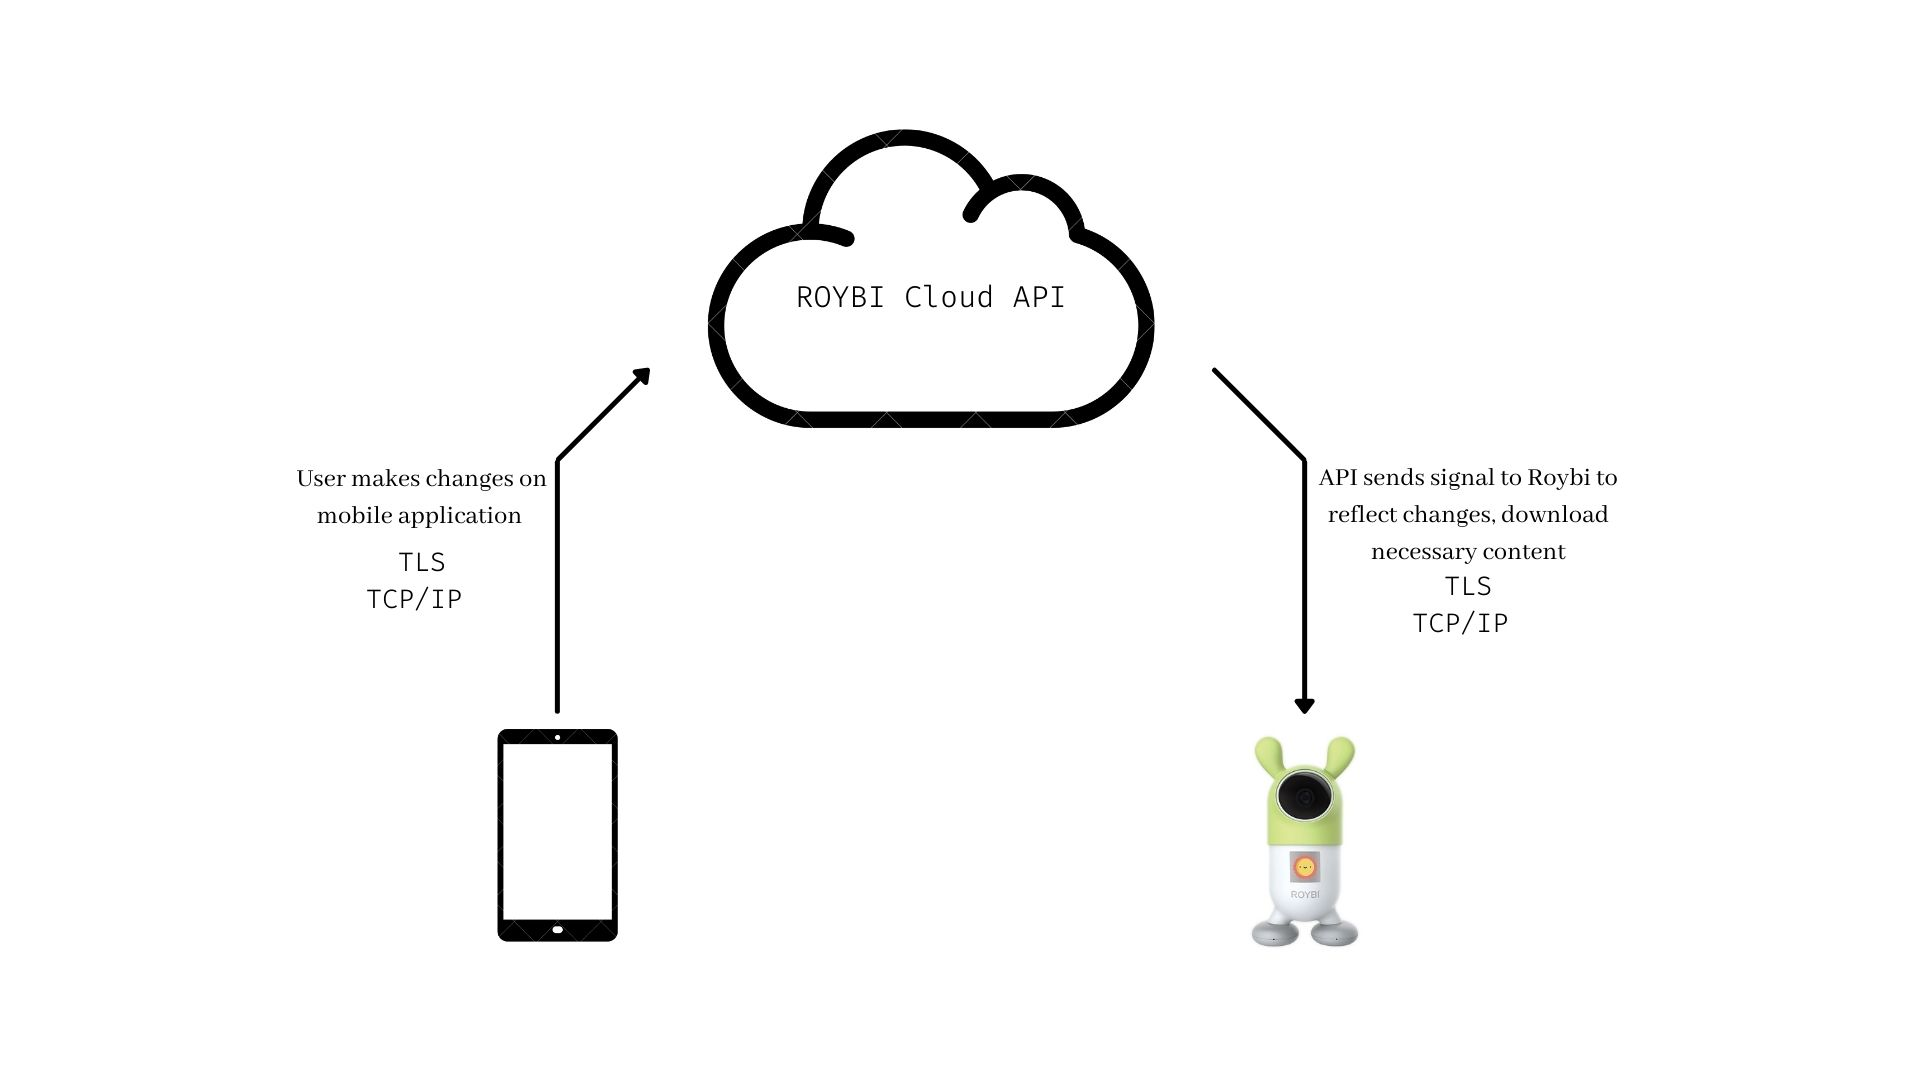
\includegraphics[width=\textwidth]{changes on app.jpg}
    \caption{Updates from the mobile application are relayed to the ROYBI device.}
    \label{fig:roybiapp}
\end{figure}

The mobile application communicates with various subdomains of \texttt{roybirobot.com} through TLS 1.2 and TCP protocols when downloading assets, making changes to a profile, and scheduling or starting lessons on the ROYBI device (fig. \ref{fig:roybiapp}). However, the Video feature on the application directly communicates with the ROYBI device through a UDP stream; when connected to the same WiFi network, our packet capture shows that the mobile device communicates directly with the ROYBI device. While on a different device, the ROYBI device streams to and from a private network address, presumably the mobile device. Through the application, the user can also speak through ROYBI's speaker, allowing a parent to communicate with the child through the device.

\begin{figure}
    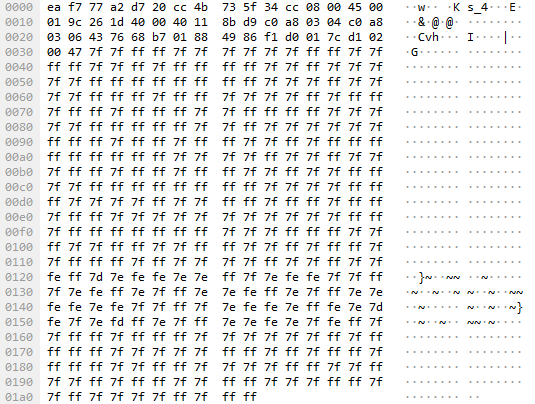
\includegraphics[width=0.5\textwidth]{unencrypted1.png}
    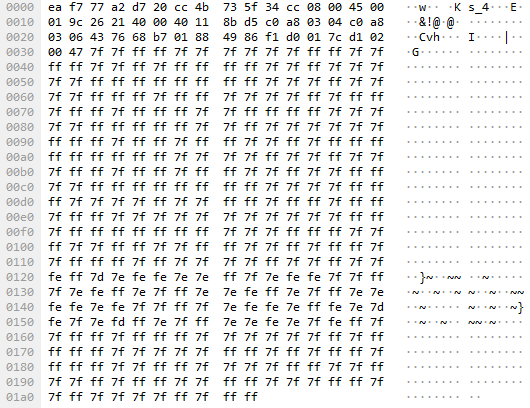
\includegraphics[width=0.5\textwidth]{unencrypted2.png}
    \caption{A Wireshark packet capture shows that the ROYBI Robot sends a UDP stream with virtually no difference in payload contents when the camera is covered.}
    \label{fig:unencrypted}
\end{figure}


\subsection{UDP Stream Analysis}
Our network analysis heavily suggests a lack of sufficient encryption for the data in these UDP packets. Again, we cover ROBYI's camera and place it in a quiet place before capturing the UDP stream. When comparing some of the identical-sized packets from the stream, we have found little to no variation between the contents of some of the packet, which indicates either no encryption, encryption key reuse, or other encryption issues. (fig. \ref{fig:unencrypted}). We first attempt to encode the payloads within the UDP packets with common media encodings. However, we have found that the beginning of each payload starts with \texttt{0xF1 D0}, which does not match the header for any common media type. Figure \ref{table:encodings} shows a list of the encodings we attempted to decode the payloads with.

Next, we perform statistical analysis on packet captures under different conditions. We capture packets from the ROYBI device both with variation in the video and audio, video without audio, audio without video, and no variation, similarly to previous experiments. With these four conditions, we calculate the statistical traits with regard to the bit at a certain index for each packet. In this experiment, we only use packets of size 1074 bytes, as only these packets showed patterns of repetition.

\begin{table}
    \centering
    \begin{scriptsizetabular}{|c|l|c|}
        \hline 
        Encoding & Description & Header or Signature \\
        \hline
        ROYBI & Unknown encoding from the ROYBI stream & \texttt{0xF1 D0} \\
        \texttt{.jpg} & Lossy compression for digital images & \texttt{0xFF D8 FF} \\
        \texttt{.png} & Digital image file type & \texttt{0x89 50 4E 47 0D 0A 1A 0A} \\
        \texttt{RTP/RTSP} & Real-time Transport (Streaming) Protocol & \texttt{b10} \\
        \texttt{.gz} & File compression format & \texttt{0x1F 8B} \\
        \texttt{.zip} & File compression format & \texttt{0x50 4B} \\
        \hline
    \end{scriptsizetabular}
    \caption{A list of common media file encodings we compared to the payloads.}
    \label{table:encodings}
\end{table}

Given the set $X_i$ of bits at index $i$ from each packet, we can find the Shannon entropy of the set
\begin{align*}
    H(X_i) = - (P(x_{i0}) \log_2 P(x_{i0}) + P(x_{i1}) \log_2 P(x_{i1})),
\end{align*}
where $x_{i0}$ and $x_{i1}$ represent the categories \texttt{0} and \texttt{1} and $P(x_{i0})$ and $P(x_{i1})$ are the probability mass functions for these categories in $X_i$. 

We used the \texttt{numpy} and \texttt{scipy} Python packages to calculate the variance and the $\chi$-squared p-value, respectively. Through Wireshark, we first apply a filter to our packet captures to show only UDP packets of size 1074 bytes sent from the ROYBI device to our mobile device. We detach the 1032 byte UDP payload from each packet; then, for each packet index, from 0 to 1031, we count the occurrences of \texttt{0} and \texttt{1} bits. For each of the indices, we calculate the Shannon entropy, variance, and $\chi$-squared values and found the average and median values across all indexed bit sets (fig. \ref{table:stats}). 

\begin{table}
    \centering
    \begin{scriptsizetabular}{|l|l|l|l|}
        \hline 
        Condition & Entropy & Variance & $\chi^2$ p-value \\
        \hline
        \hline
        \textbf{Video and audio} & & & \\
        Average & 0.9803676240724125 & 0.2438377782554819 & 0.06999612094542865 \\
        Median  & 0.9937492975910669 & 0.2478368020888454 & 5.798602844885254e-17 \\
        \hline
        \hline
        \textbf{Video, no audio} & & & \\
        Average & 0.985552608626217  & 0.2455559533577817 & 0.0382156014086419 \\
        Median  & 0.9910639794988954 & 0.2469094108184754 & 1.0495224726537987e-49 \\
        \hline
        \hline
        \textbf{No video, audio} & & & \\
        Average & 0.7047054527908376 & 0.1642110854920916 & 0.05488155260850076 \\
        Median  & 0.7743757078053616 & 0.1759749377002492 & 2.5705208923537022e-87 \\
        \hline
        \hline
        \textbf{No video, no audio} & & & \\
        Average & 0.8508982500756426 & 0.20492332037463712 & 0.04328112347390702 \\
        Median  & 0.8939252655352993 & 0.21414753850025312 & 7.476376446385691e-114 \\
        \hline
    \end{scriptsizetabular}
    \caption{Results of a statistical analysis of the UDP stream.}
    \label{table:stats}
\end{table}

From our results, we found that the entropy and variance on streams with the ROYBI device's camera uncovered was noticeably higher than those where the camera was covered. Furthermore, the $\chi^2$ p-values we found shows high confidence levels for our reported values. Given that we found repeating patterns from camera-covered streams, our statistical analysis shows the different distributions of bits between noisy data and consistent data; if the data was well encrypted, we would expect to find little difference in these values.

Finally, we measure the bandwidth of the UDP stream under the same conditions and compare our results. As found in previous research by Valente et al. \cite{valente}, a traffic analysis may show information leakage depending on the differences in bandwidth and packet transmission rate. In Wireshark, we apply a filter to our packet capture to only show UDP packets sent from the ROYBI device to our mobile device. Then, with the \texttt{dpkt} Python package, we parse the payload and timestamp from the filtered packet capture, binn each packet by seconds from the timestamp of the first packet, and fit the data to form our graphs (fig. \ref{fig:plots}). We found that streams containing dynamic video data transmitted noticeably more packets and had higher bandwidth compared to streams where the device's camera was covered. Additionally, we found that the absence of dynamic audio increased the bandwidth and packet transmission rate while a noisy environment decreased them.

\begin{figure}
    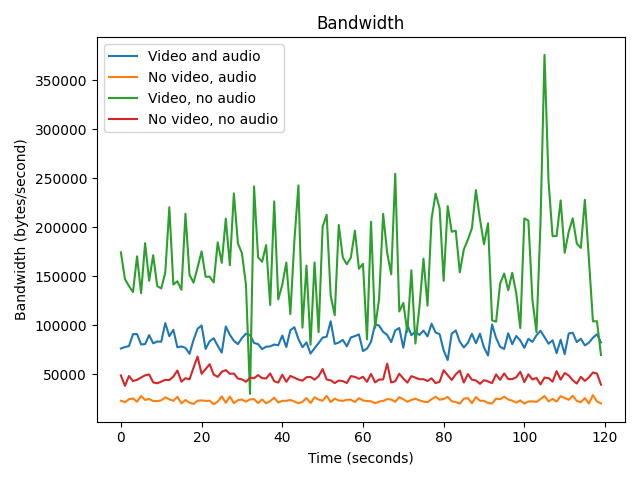
\includegraphics[width=0.5\textwidth]{bandwidth.png}
    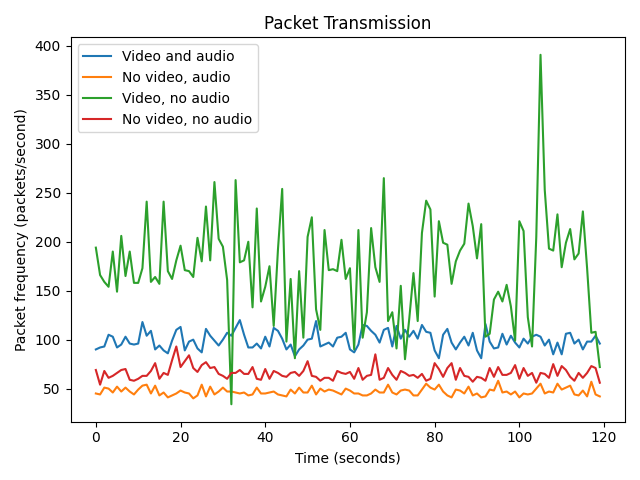
\includegraphics[width=0.5\textwidth]{packettrans.png}
    \caption{A measure of the UDP stream bandwidth and packet transmission rate under different conditions.}
    \label{fig:plots}
\end{figure}

\subsection{ROYBI Robot Attack Vectors}

\subsubsection{Credential Stuffing}
\begin{figure}
    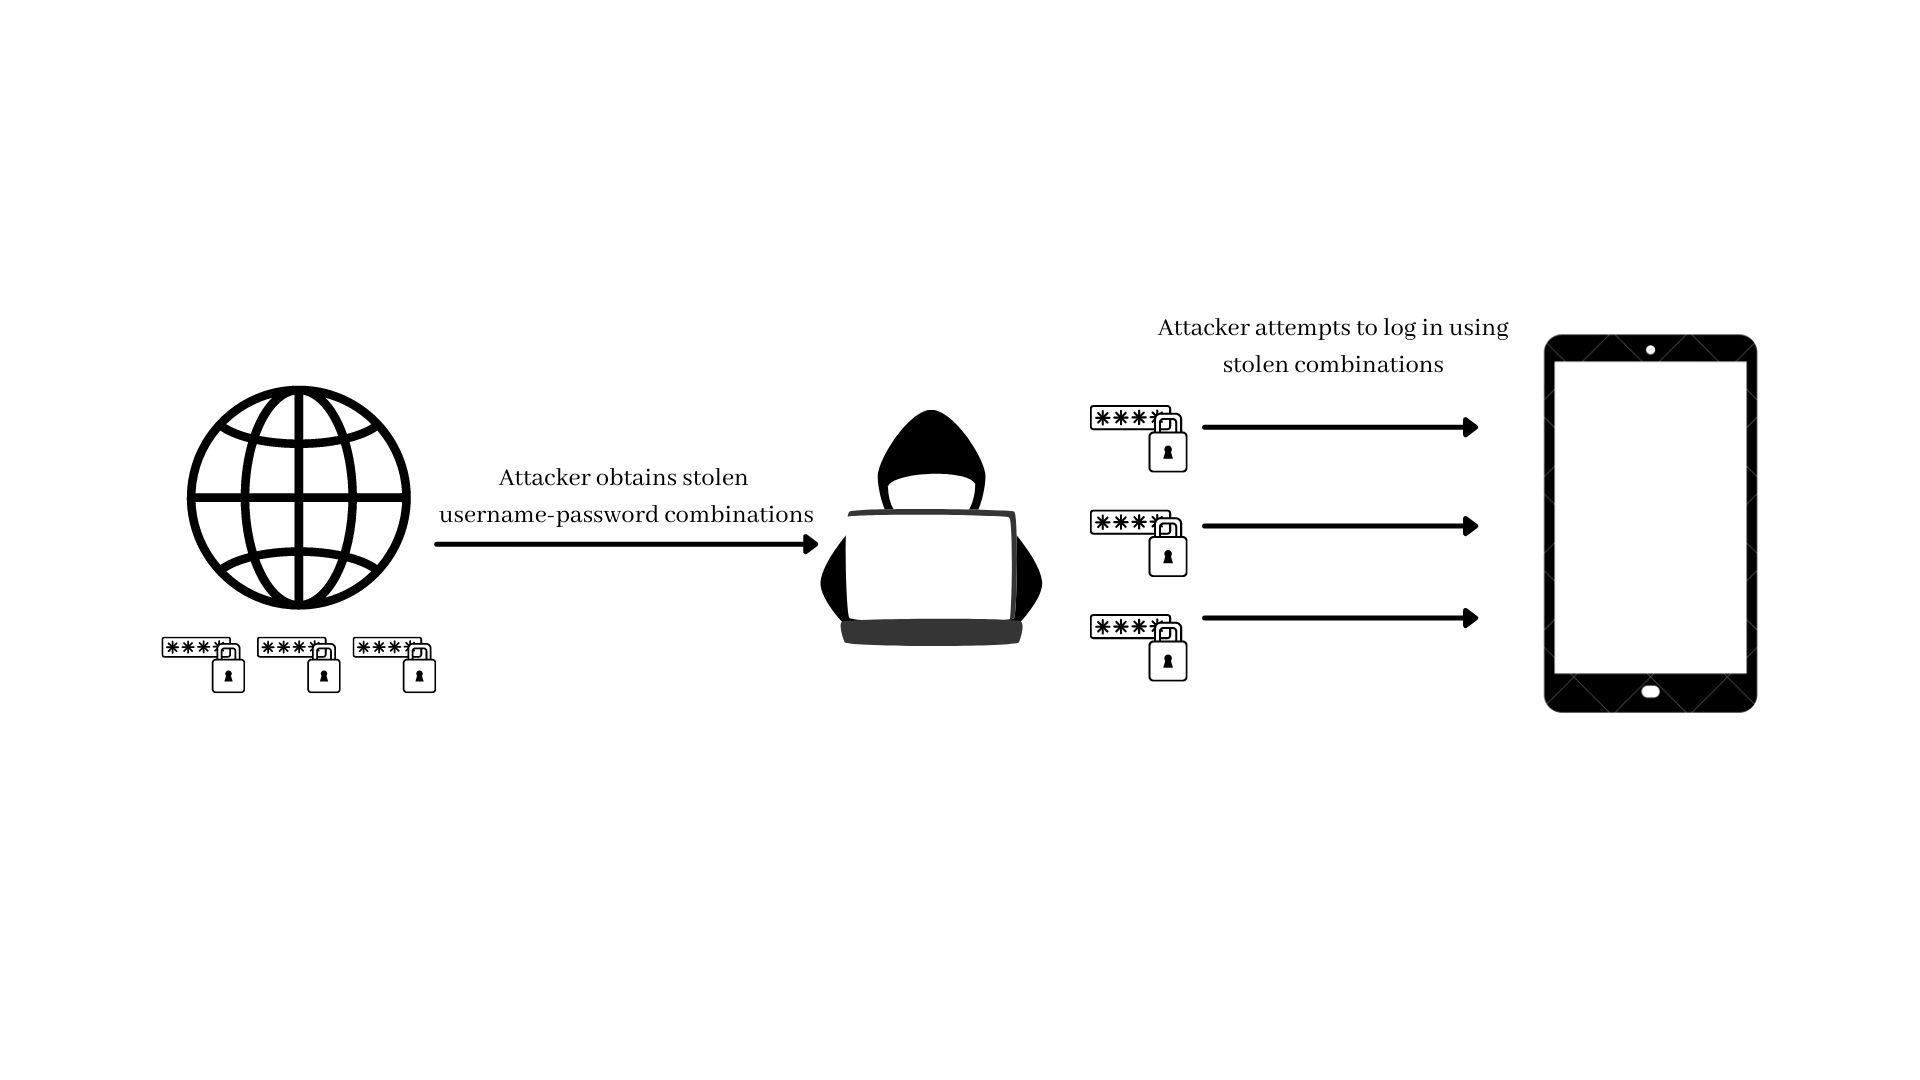
\includegraphics[width=\textwidth]{stuffing.jpg}
    \caption{Adversaries can perform a credential stuffing attack by obtaining username-password combinations and repeatedly attempt log ins.}
    \label{fig:stuffing}
\end{figure}

Similar to the issue that the Amazon Echo Dot faces, if a ROYBI user's credentials are compromised, they are at risk of having their account breached. The ROYBI mobile application does not implement any further security measures for repeated login attempts, meaning their system is fully susceptible to credential stuffing attacks (fig. \ref{fig:stuffing}) \cite{stuffing}. Upon breach, attackers gain access to all profile information and can alter lesson schedules. Moreover, attackers can use the Video feature to access the camera and video feed as well as communicate directly with anyone present with the ROYBI device.

\subsubsection{Spying}
We cite Kerckhoffs' Principle \cite{kerckhoffs} to address the issues we found with ROYBI's Video feature; when designing a secure system, parties should rely on only its choice in cryptographic keys to maintain secrecy. In ROYBI's case, we found pooly encrypted UDP streams that contained video and audio data (fig. \ref{fig:unencrypted}). While the streaming protocol is unknown, in the event where an attacker discovers how these streams are processed, they will have full access to the video and audio between the two devices, presenting a severe security risk (fig. \ref{fig:evesdropper}).

\begin{figure}
    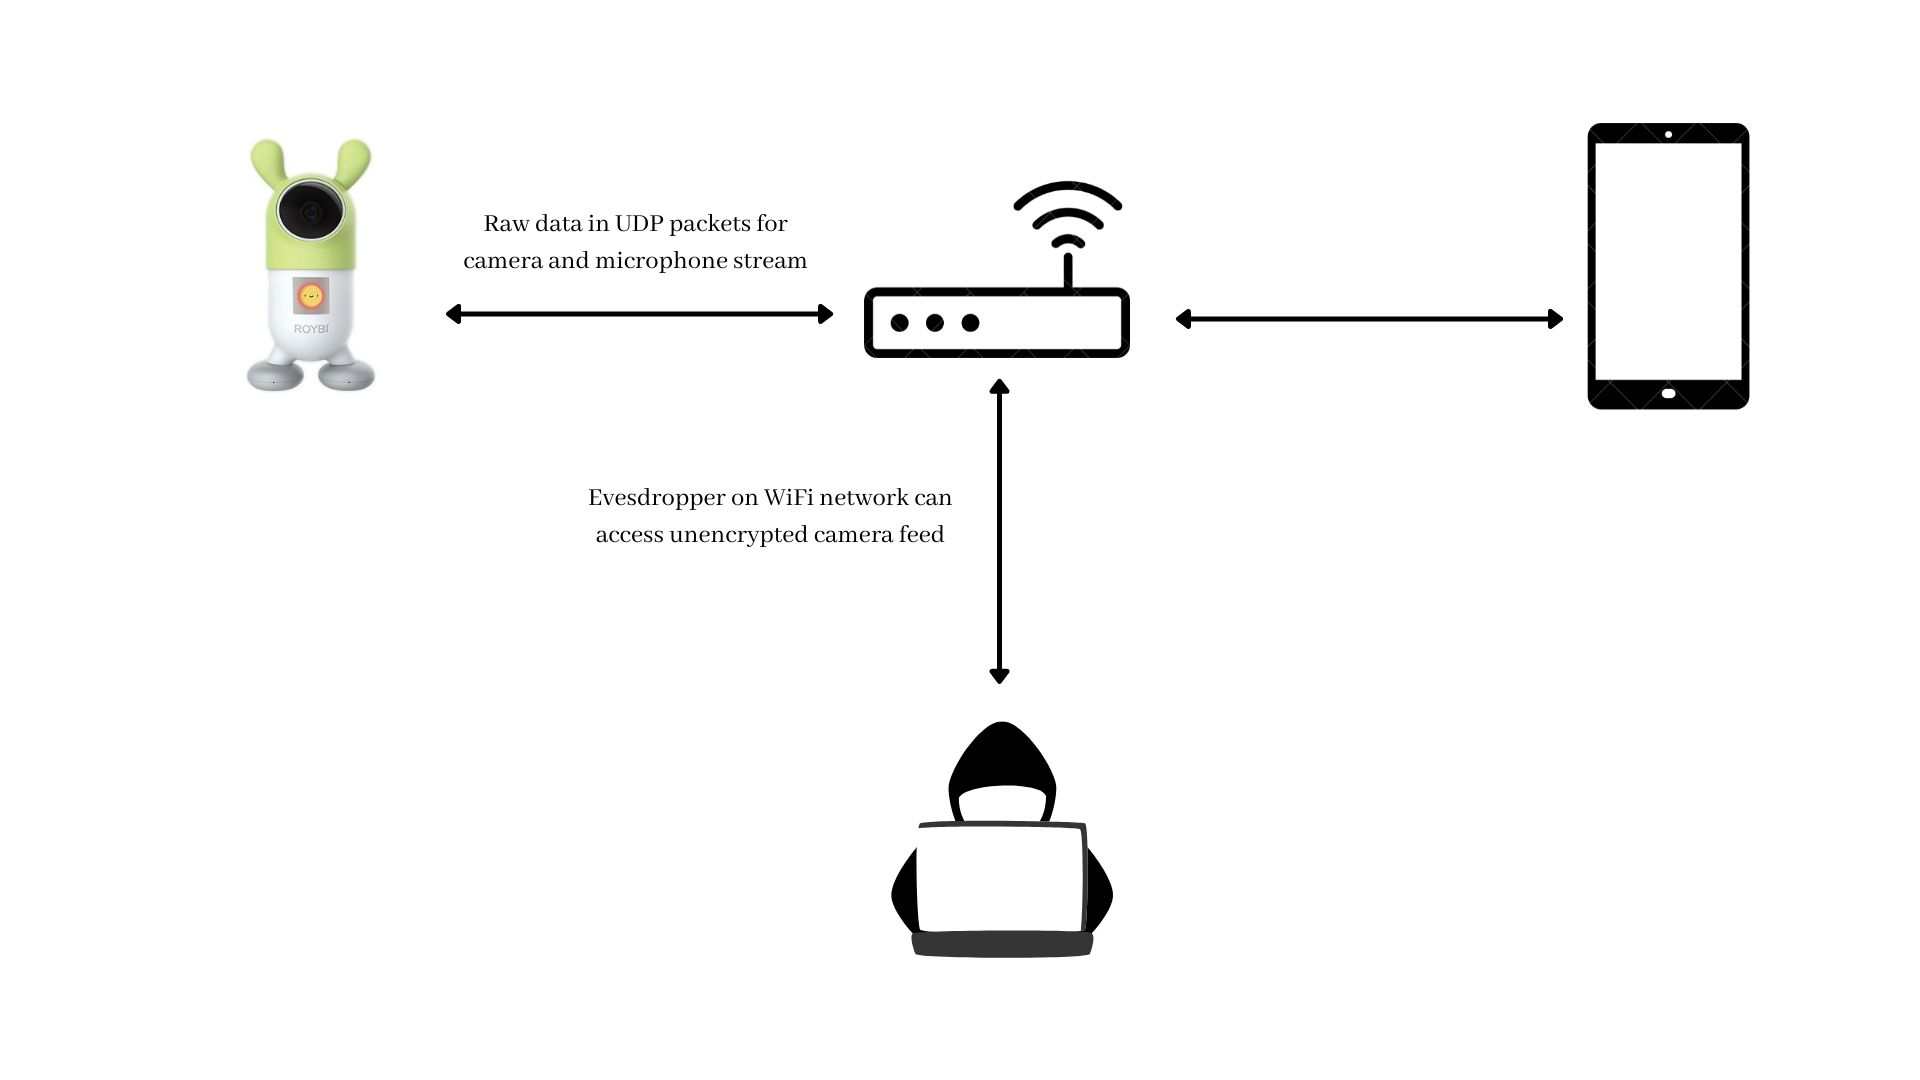
\includegraphics[width=\textwidth]{evesdropper.jpg}
    \caption{Adversaries on the same WiFi network as ROYBI have access to poorly encrypted camera and microphone feed data.}
    \label{fig:evesdropper}
\end{figure}

% CONCLUSION %%%%%%%%%%%%%%%%%%%%%%%%%%%%%%%%%%%%%%%%%%%%%%%%%%%%%%%%%%%%%%%%%%%%%%%%%%
\chapter{Conclusion}
\label{ch:conclusion}
Based on our finding and survey data, we make some recommendations for IoT developers. We also delve into future work to further develop our models.
\section{Recommendation}
\subsubsection{Preventing Automated Attacks}
As we have observed from the Alexa mobile application, users are required to complete a CAPTCHA challenge after multiple failed log in attempts. This was not a security feature that was implemented in the ROYBI mobile application, and thus exposed ROYBI's system to large-scale automated attacks, such as credential stuffing, brute force attacks, and dictionary attacks \cite{brute}. In any service that requires logging in, we recommend that developers implement a similar mechanism to prevent attacks like these.

\subsubsection{Multi-Factor Authentication}
Research has shown that MFA adds a nearly inpenetrable layer of security to an authentication system \cite{mfa}. While it can be hard to convince users to take an extra step before being able to log into their accounts, developers should at least provide an option to allow users to enable MFA. Ideally, this should be required for all users to ensure maximum security in the system; for example, the University of California has recently required all students and faculty to use Duo, a MFA service, to access their university accounts. 

\subsubsection{Encrypt Everything}
In our network analysis, we have found that the ROYBI device does not securely encrypt all of its outgoing packets. Currently, the payload of these packets contain similarly-patterned data and holds no indicator of which media protocol is used to process it. However, in the event that an attacker gains knowledge of how the stream is processed, they are easily able to see and hear all video and audio data that the ROYBI device sends. We recommend that \textbf{all} network traffic should be encrypted using a strong encryption algorithm to prevent privacy breaches in the future.

\subsubsection{Data Collection Transparency}
We have found in our survey data that many consumers are often reluctant in using smart devices because of a lack of understanding in what data is collected and how it is stored. Prior research has found that the vast majority of people do not read privacy policies at all \cite{privacypolicy}, so developers can reasonably expect that users are not fully aware of any data collection occurring. To remedy this problem, developers should take more initiative in informing users of their data collection methods. 

\section{Future Work}
As IoT is still a growing industry, there are still more vectors to explore within this field. Since there are many more smart devices on the market, we can perform network analysis on a different set of devices and compare them to our findings in this research. Prior research has found many more security issues present in other smart toys \cite{cardenas:smarttoys}, which leads us to believe that children's IoT devices are lacking in security development.

We also aim to further diversify our survey participants. Most of our participants were contacted through word of mouth or chosen from an existing subject pool, courtesy of the Baby Lab at UCSC. By reaching out to a wider variety of people from different background, we can form a more thoroughly developed mental model for parents and IoT devices, which in turn gives us a better look at what recommendations to make for developers.

Instead of a survey, our original plan was to interview parents and children in-person. In this setting, we also allow the child to interact with the devices. This method of data collection should have provided parents with more insight on how these devices work and provided us with the child's viewpoints as well. While in-person data can be more valuable to our research, we unfortunately could not conduct these interviews due to the COVID-19 pandemic. In the future, we will have the ability to look into children's opinions on the matter as well. From here, we can also build a mental model for children in addition to the parents.

%Finally, although it is likely that these packets are unencrypted, we did not fully delve into the UDP streams captured from the ROYBI Robot in this paper. In future developments, there are various ways to analyze this data. For example, we can perform statistical analysis on the differentiation between like-sized packets in order to measure the randomness of the data. We can also attempt to encode the raw data by adding media file headers to try to find how the devices process this data. With further analysis, we can better understand the extent of encryption, if any at all, used in the device's backend.

\section{Conclusion}
Throughout this thesis, we have explored data privacy, security mechanisms, and consumer insights on smart devices designed for children. In developing a generalizable mental model of parents who allow their children to use smart devices, we are able to better understand the security practices these parents neglect, what concerns they have regarding cloud infrastructures, and what weaknesses must be strengthened for a more secure IoT environment.

We were able to find security concerns and attack vectors by performing network analyses on the ROYBI Robot and the Amazon Echo Dot for Kids. From here, we develop a threat model to accompany the mental model. By comparing the two, we find solutions to the issues we found within the IoT framework. Finally, we aim to provide recommendations for IoT developers in order to ensure the security and privacy of consumers and their children.

% BIBLIOGRAPHY %%%%%%%%%%%%%%%%%%%%%%%%%%%%%%%%%%%%%%%%%%%%%%%%%%%%%%%%%%%%%%%%%%%%%%%%
\nocite{*}
\bibliographystyle{plain}
\bibliography{uctest}


% APPENDIX %%%%%%%%%%%%%%%%%%%%%%%%%%%%%%%%%%%%%%%%%%%%%%%%%%%%%%%%%%%%%%%%%%%%%%%%%%%%
\appendix
\chapter{Survey Questions}
\label{app:questions}
The following section contains the questions we ask in our survey. Some topics include experience with technology, perceptions of our subject devices, data privacy, and demographics.

\begin{itemize}
    \item Smart device related questions
    \begin{itemize}
        \item If you own a smart home device, how long have you been using it?
        \item Does your child have access to a smart home device?
        \item If you own any other smart devices (e.g. smart watch, smart TV, etc.), how long have you been using it?
        \item Does your child use smart devices other than smart home devices?
        \item If you do \textbf{not} own any smart devices, would you consider buying one? Will your child have access to it? Why or why not?
    \end{itemize}
    \item Subject device questions
    \begin{itemize}
        \item Have you heard about this toy/device? If yes, please explain where.
        \item What do you like about the toy/device?
        \item What do you dislike about the toy/device?
        \item Would you consider purchasing the toy/device? If so, why? If not, what kind of improvements would you like to see be made for you to reconsider?
        \item What do you expect to be in the toy/device's privacy policy?
    \end{itemize}
    \item Scale questions (scale on Disagree-Agree)
    \begin{itemize}
        \item I have concerns for how my data is collected and stored on the Internet.
        \item I find it important that collected data is kept private.
        \item I thoroughly research into Internet-connected devices before making a purchase.
        \item I am familiar with the Children’s Online Privacy Protection Act (COPPA).
    \end{itemize}
    \item Data privacy questions
    \begin{itemize}
        \item Please describe your understanding of how Internet-connected devices collect data. 
        \item Please describe your understanding of where and how this data is stored.
        \item Please describe any concerns for how your data is stored on the Internet.
        \item What practices does your family use to keep your data safe?
        \item Have you had any security concerns with devices connected to the Internet?
        \item What concerns do you have about the dialogue between your child and the devices presented in this survey?
    \end{itemize}
    \item Demographics questions
    \begin{itemize}
        \item Age 
        \item Age(s) of children 6 years old or younger
        \item Highest level of education
        \item Occupation
        \item Family household income
        \item Experience with technology
    \end{itemize}
  \end{itemize}
\end{document}
